\documentclass{jfm}
\usepackage{graphicx}
\usepackage{epstopdf, epsfig}
\usepackage{lipsum}
\usepackage{gensymb}
\usepackage{booktabs}
\usepackage{makecell}
\usepackage{multirow}
\usepackage{float}
\usepackage{color}
\usepackage{tikz}
\usetikzlibrary{shapes}
\usepackage{amsmath}
\shorttitle{Liquid chain genesis}
\shortauthor{V. Sanjay and A. K. Das}
\title{Liquid Chain Genesis by Collision of Two Laminar Jets}
\author{Vatsal Sanjay,
  Arup K. Das\corresp{\email{arupdas80@gmail.com}}}
\affiliation{Department of Mechanical and Industrial Engineering, Indian Institute of Technology, Roorkee}

\begin{document}
\newcommand{\MarkerCircleRed}{\raisebox{0.5pt}{\tikz{\node[draw,scale=0.4,circle,fill=red!100!red](){};}}}
\newcommand{\MarkerSquareRed}{\raisebox{0.5pt}{\tikz{\node[draw,scale=0.4,regular polygon, regular polygon sides=4,fill=black!20!red](){};}}}
\newcommand{\MarkerDiamondBlack}{\raisebox{0pt}{\tikz{\node[draw,scale=0.4,diamond,fill=black!100!](){};}}}

\maketitle
\begin{abstract}
\end{abstract}
\lipsum[1]
\begin{keywords}
\end{keywords}
\section{Introduction}
Interactions of liquid jets have invoked the curiosity of researchers with their ubiquitous presence, eminent even in the scientific artworks by Leonardo Da Vinci in the 16$^{th}$ century. Physics of different types of interactions related to liquid jets is classically summarized in a recent effort by \cite{eggers2008physics}. One of these interactions is the collision between liquid jets, presented by \cite{rayleigh1879capillary}. \cite{bush2004collision} introduced several regimes to characterize the different flow structures obtained from such collisions, working on the theory of liquid jet impingement given by \cite{taylor1960formation}. At low velocities or narrow angles of impingement, jets may coalesce to form a unified one or bounce off due to presence of a thin film of air between them \citep{wadhwa2013noncoalescence}. On increasing the flow rates, laminar jets may lead to formation of a stable liquid sheet bounded by a thick rim \citep{yang2014liquid}. Inertia and gravitational forces act to expand the liquid sheet formed but the action of surface tension puts a check and allows the sheet  to converge, such that the successive collisions of the thick rims downstream of the flow result in formation of mutually orthogonal liquid sheets \citep{bush2004collision}. Figure~\ref{Figure::schematic}a illustrates this structure termed as the liquid chain with the complementary orthogonal sheets forming the different links. Alternatively, further increase in jet velocity, due to several instability modes, leads towards ejection of droplets from the liquid rim \citep{bremond2006atomization}, fluid fishbones \citep{bush2004collision} and flapping sheet \citep{villermaux2002life} associated with atomized drops \citep{ibrahim1991impinging}. The stable chain regime is not just an idealization of the violent flapping, but also holds physical significance for the exploration of fundamental physics behind atomization. Moreover, these structures can be used as wall-free continuous reactors \citep{erni2013free} and are often used as a canonical arrangement for generation of liquid sheets \citep{dombrowski1954photographic}. \\
\begin{figure}
	\centering
	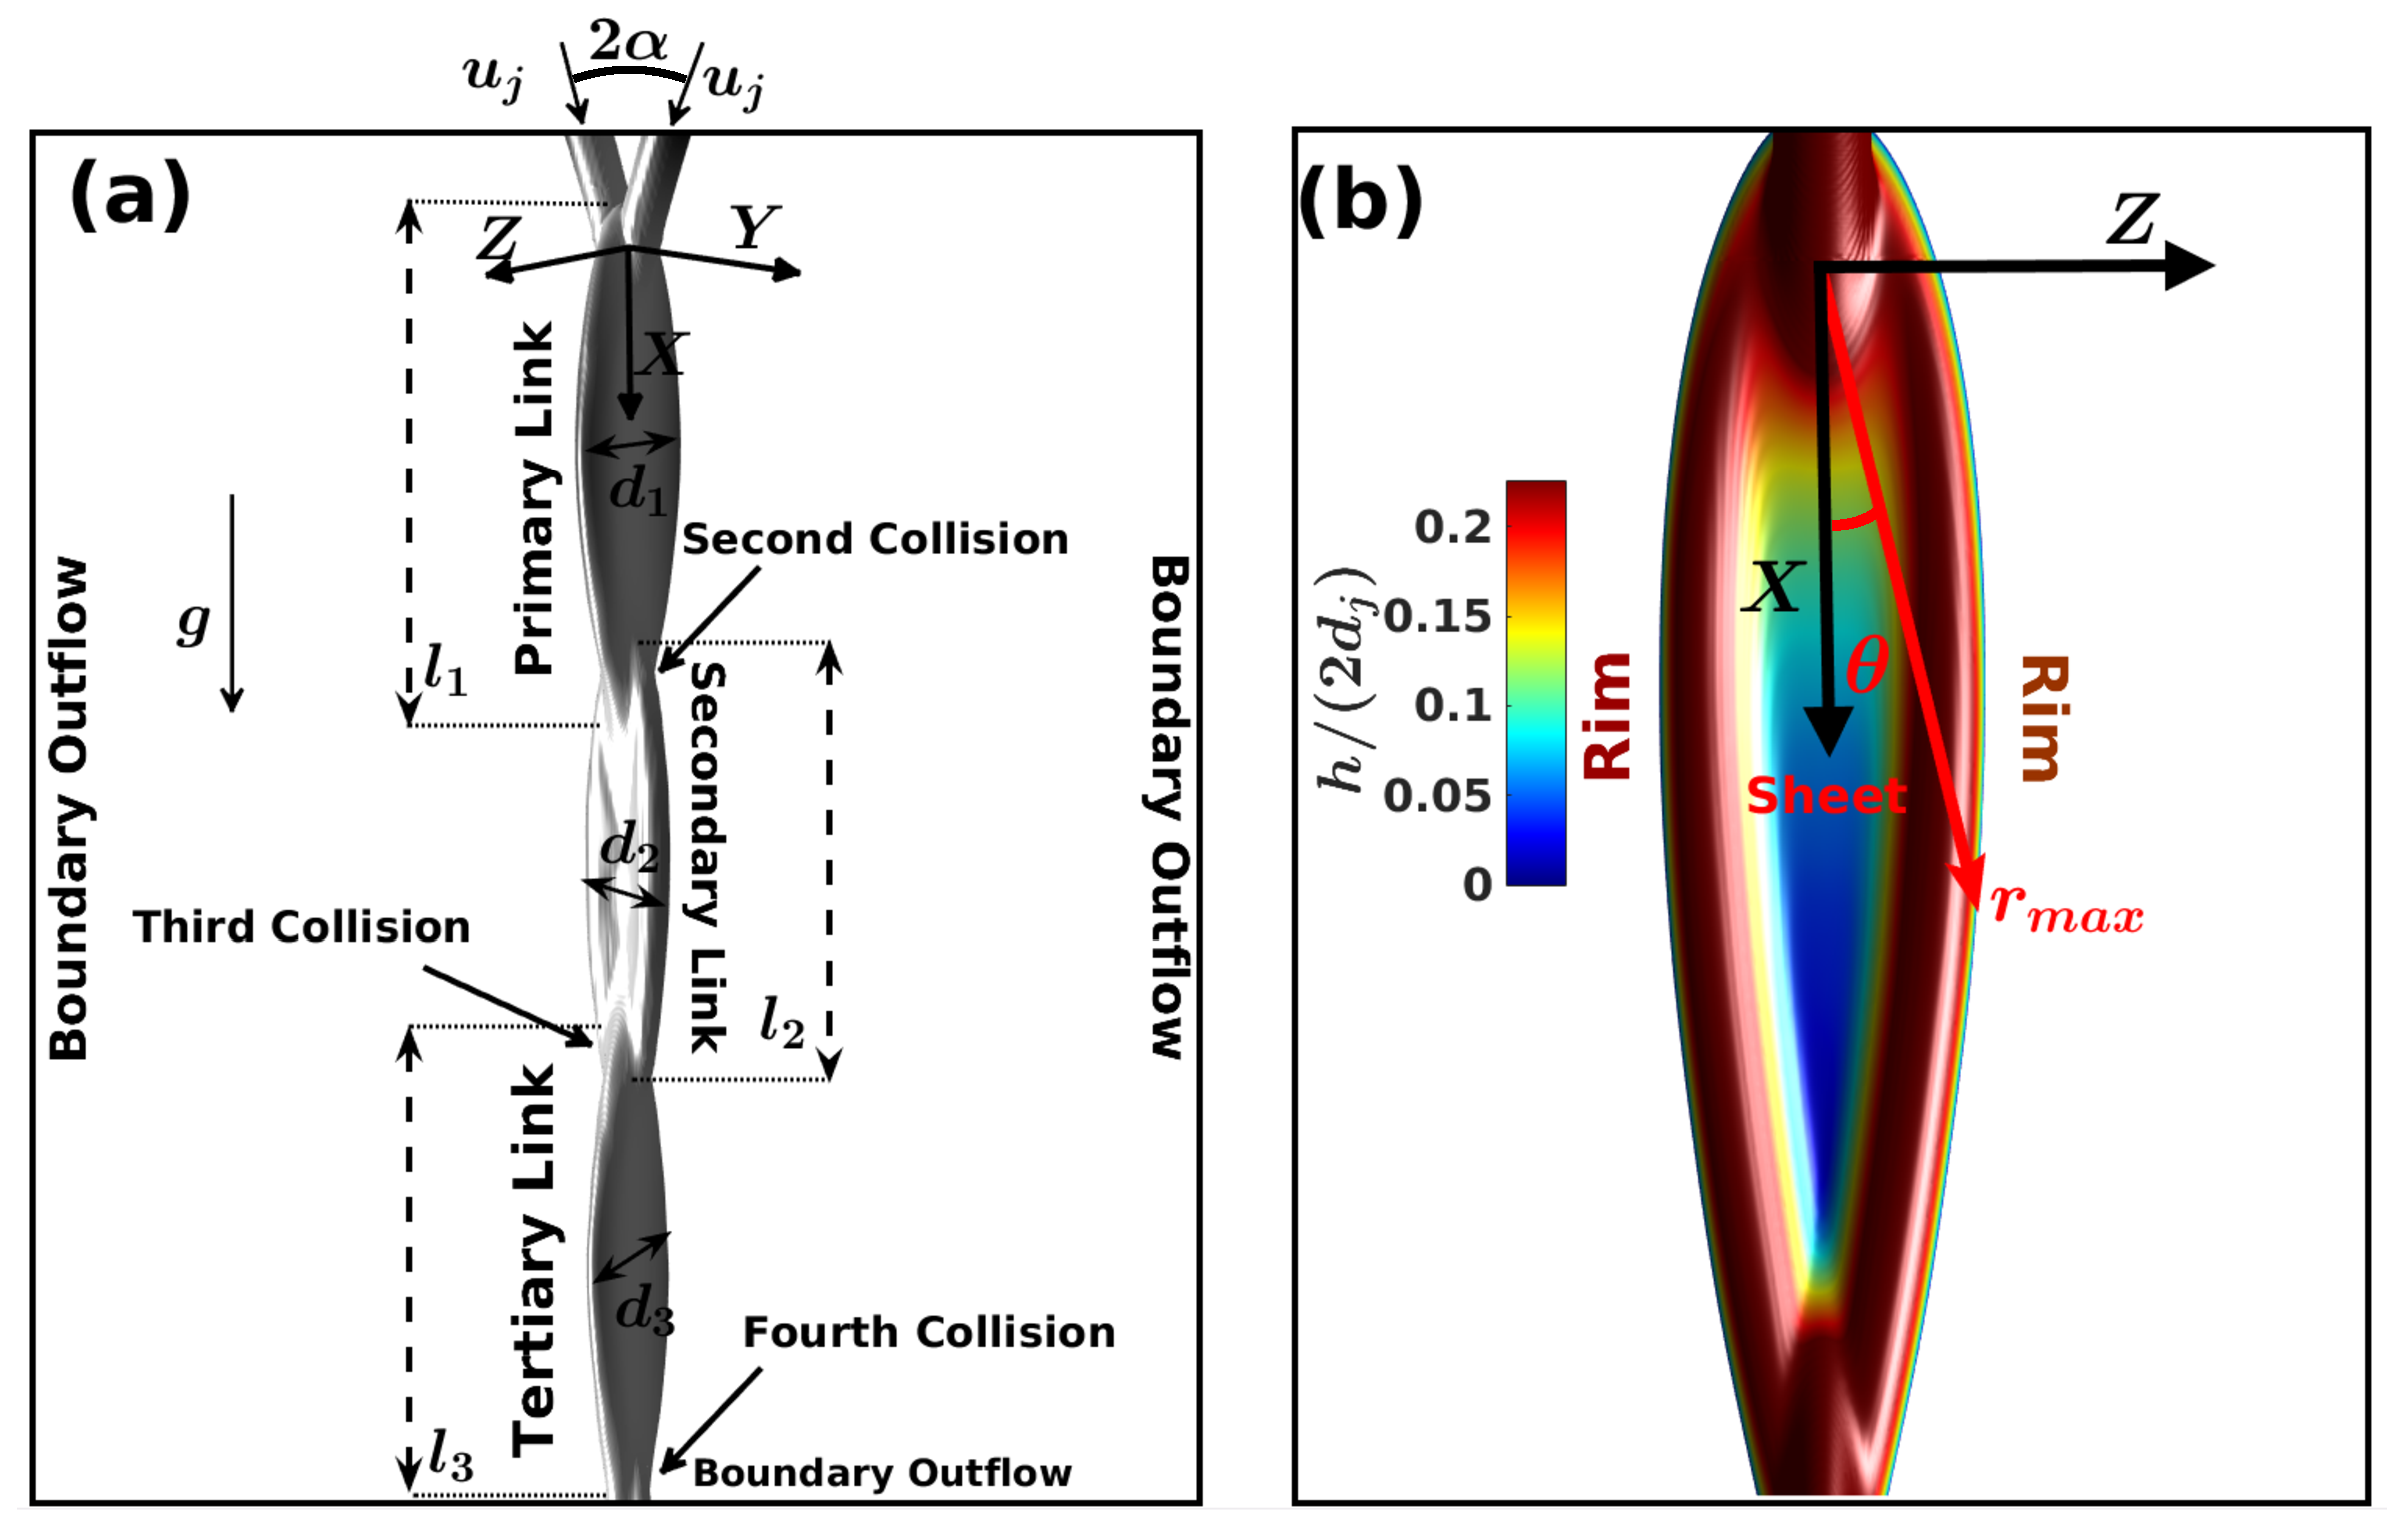
\includegraphics[width=0.6\linewidth]{Figure1}
	\caption{Formation of the liquid sheet by collision of laminar jets. (a) A schematic to illustrate different structural features and length scales. The mutually perpendicular sheets mark different links of the fluid chain structure. (b) The primary link structure colored based on half times the magnitude of the sheet thickness, non-dimensionalized with the jet diameter ($\frac{h}{2d_j}$).}
	\label{Figure::schematic}
\end{figure}
Keeping this fascinating applications in mind, a range of  experimental works can be found exploring the formation of stable liquid sheets using viscous jets \citep{choo2001parametric,choo2002velocity,bush2004collision}. Using Particle Image Velocimetry (PIV) technique, radial streamlines are observed near the point of impingement and the fluid parcels travel towards the periphery resulting in the formation of the thick rim due to fluid accumulation \citep{choo2002velocity,bush2004collision}. The rim is stable as long as the curvature force developed by surface tension provides the necessary centripetal acceleration as the fluid packets in the rim accelerate owing to loss in gravitational potential \citep{bremond2006atomization}. On balancing the two, \cite{taylor1960formation} developed an expression for the sheet radius which has been found to describe the experimental results of \cite{bush2004collision} reasonably well. Emphasis has been also given by \cite{bush2004collision} for prediction of shapes of leaf like links forming chain structure. However, the model requires input from the experiments so as to close the system of differential equations. Isolated numerical efforts are also found describing different possible outcomes due to liquid jets interactions. As a part of their study, \cite{chen2013high} have shown formation of liquid chain using Finite Volume based Volume of Fluid (VOF) network. Recently, \cite{da2016surface} also demonstrated formation of liquid chain using Boundary Element Method (BEM). But, their exhibition of chain like structure along with other physical jet related structures suffer from inviscid assumption.\\
Critical assessment of literature reveals that an in-depth study of fluid chain regime is still due which can explore fundamental physics behind formation of primary link and establish relation between successive diminishing links. Major challenge that lies in the prediction of chain like structure is the proper resolution of sheet (approximately $1/100^{th}$ of jet diameter) between the rims, which are supposed to mingle once again for forming next link in mutually perpendicular plane. Figure~\ref{Figure::schematic}b is presented to demonstrate the presence of a range of length scales in such a simplistic fluid link. In the present work, we attempt at study of an overall behavior of the fluid chain  while focusing on the physics of flow for the primary link by analyzing the dimensional characteristics and velocity fields. Special attention is given to the second and third collisions, leading to the formation of the subsequent mutually orthogonal links and relate them from fundamental force balance. In the next section, the numerical framework employed in this work is briefly explained before reporting mesh sensitivity analysis and validation.
\begin{figure}
	\centering
	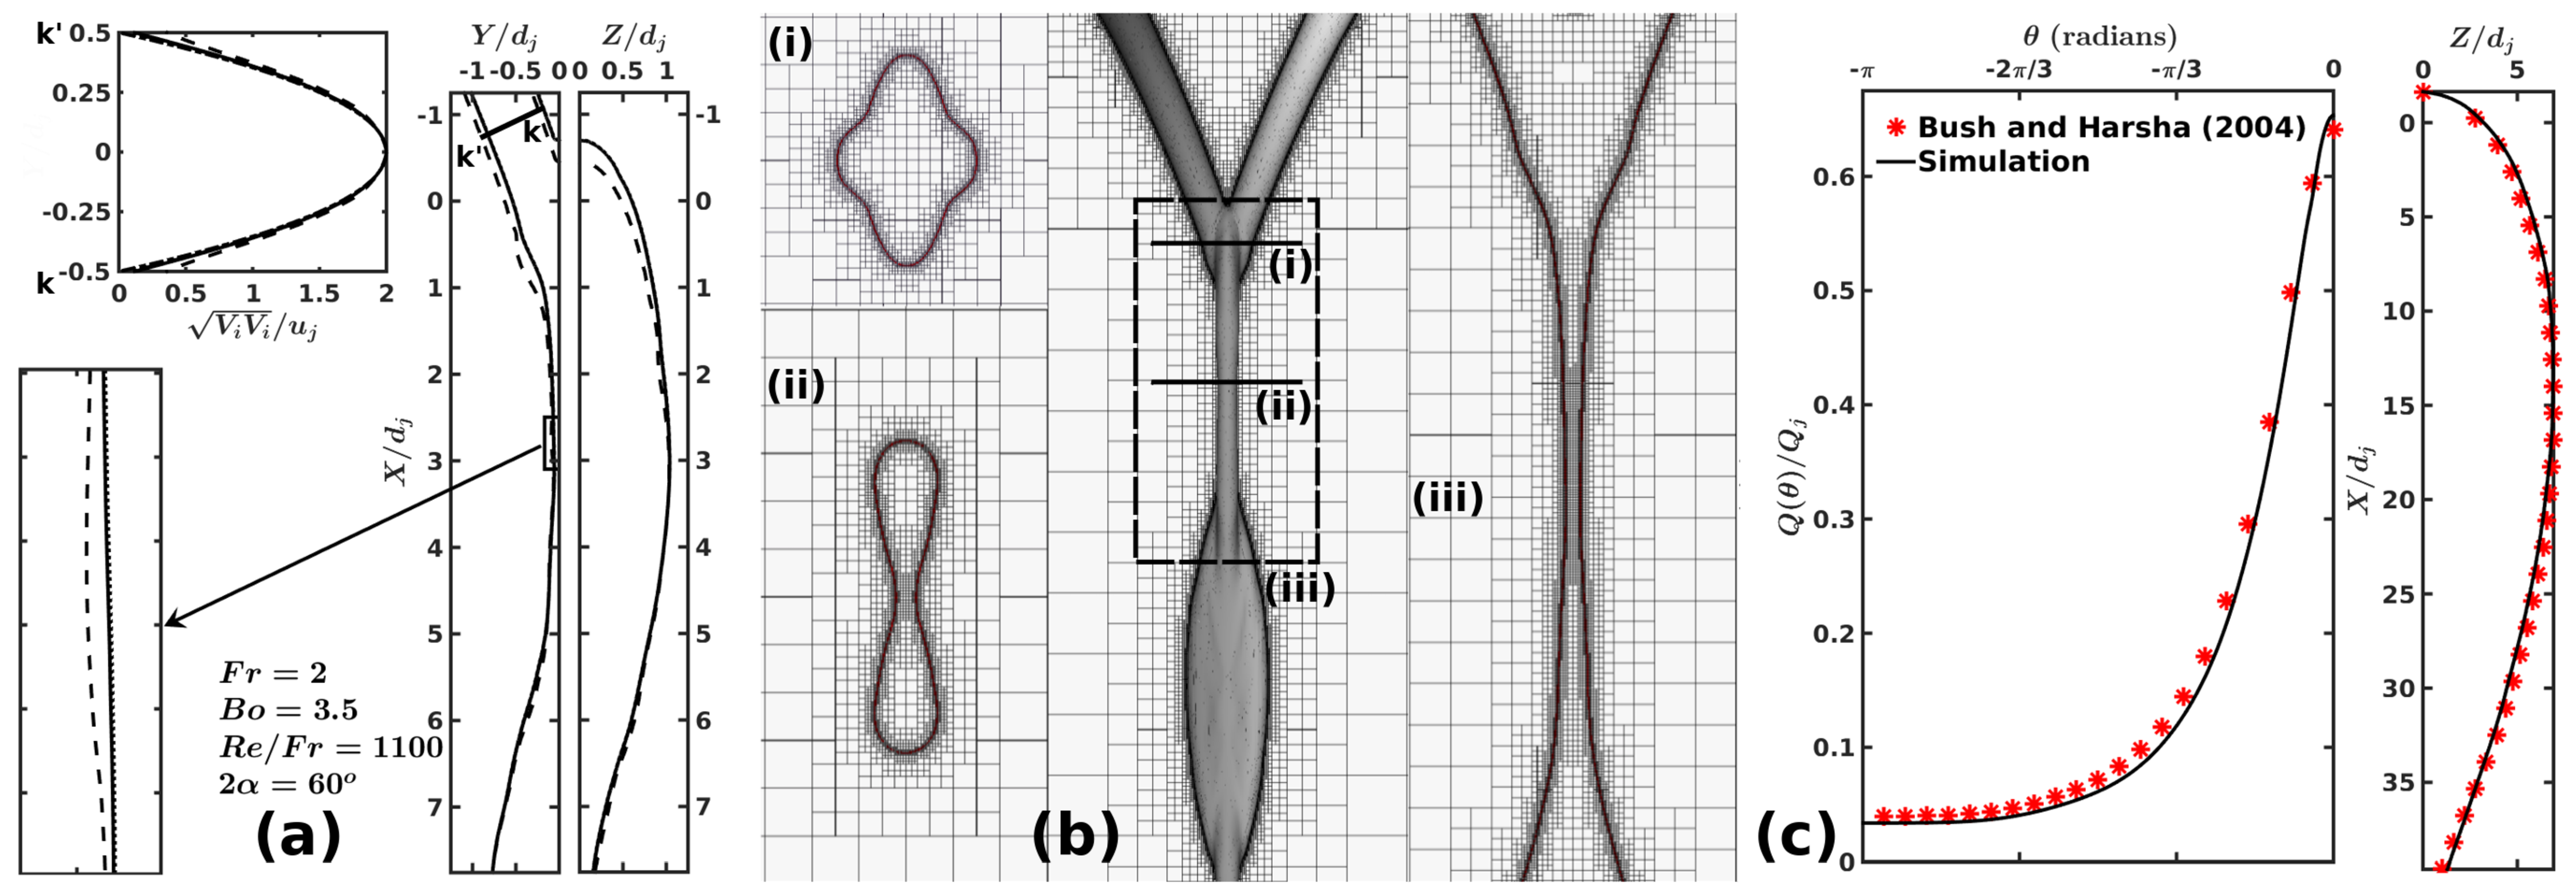
\includegraphics[width=\linewidth]{Figure2}
	\caption{(a) Mesh Sensitivity Analysis for a representative chain structure with outer periphery and velocity profile near the inlet; (b) Representation of the Adaptive Mesh Refinement (AMR) technique at critical locations; (c) Numerical interface (left) and Liquid flux (right) superimposed with the respective experimental values obtained by \cite{bush2004collision} to depict validation.}
	\label{Figure::gisetal}
\end{figure}

\section{Numerical framework}
Collision of liquid jets has been studied in three-dimensional  finite volume framework. Open source, time-dependent, multi-fluid, Navier-Stokes solver, Gerris is used for the current study \citep{Popinet2003}. The spatial discretization of the domain is undertaken using an octree based structured hierarchical grid system, locally refined near the interface. Conventional mass and momentum conservation equations for incompressible flow have been solved in presence of interface specific surface tension force ($\sigma \kappa$, where $\sigma$ is the surface tension coefficient and $\kappa$ denotes the curvature of the interface) and gravitational field ($\rho g$). The interface tracking is undertaken using the Volume Of Fluid (VOF) approach using volume fraction of liquid, defined as $\Psi(x_i, t)$, at the spatial and temporal instance of $x_i$ and $t$ respectively. Therefore, the density and viscosity for the study can be described using Equation~\ref{Equation::general}.
\begin{equation} \label{Equation::general}
A (\Psi) = \Psi A_1 + (1-\Psi)A_2 \: \: \:  \forall  \: A \in \{\rho, \mu\}
\end{equation}
The VOF approach is implemented in a two-step process of interface reconstruction (based on the values of $\Psi$ and piecewise linear interface construction scheme, PLIC) along with geometric flux computation and interface advection, shown in Equation~\ref{Equation::vof}.
\begin{equation} \label{Equation::vof}
\frac{\partial \Psi}{\partial t} + \frac{\partial(\Psi V_i)}{\partial X_i} = 0
\end{equation}
Gerris uses second order accurate time discretization of momentum and continuity equations with time splitting algorithm as proposed by \cite{Chorin1968}, whereby an unconditionally stable corrector predictor time marching approach is adopted. A multi-grid solver is used for solution of the resulting pressure-velocity coupled Laplace equation. The advection term of the momentum equation $\left(V_k\frac{\partial V_i}{\partial X_k}\right)$ is estimated using the Bell-Colella-Glaz second-order unsplit upwind scheme \citep{bell1989second}, which requires the restriction to be set up on the time step. Following \cite{popinet2009}, time step has been determined to satisfy Courant-Friedrich-Lewy (CFL) stability criteria of less than unity. The details of solution procedure can be found in the works of \cite{Popinet2003,popinet2009}.\\
The computational domain is also illustrated in Figure~\ref{Figure::schematic}a with parabolic inflow (average velocity, $u_j$) of jets (diameter, $d_j$ and impingement angle, $2\alpha$) and boundary outflow elsewhere. From the works of \cite{choo2001parametric}, it can be easily shown that the thickness of liquid sheet follows $\frac{hr}{d_j^2} \sim 1$, for $2\alpha \in \{0,\pi/2\}$.  Here, $r$ is the radial direction originating from the collision point of the jets and h is the measurement of thickness of the film produced by jet collision. We maintained $\frac{d_j}{\delta l} \sim 10\frac{r_{max}}{d_j}$ to choose minimum cell size $\left(\delta l\right)$ and perform Grid Independence Study (GIS). The factor of 10 is included to have at least 10 grid points\citep{ling2015multiscale} across the smallest length scale for the structure to avoid breakage of sheet \citep{chen2013high}. To obtain continuous liquid film and well resolved phenomenon, $\delta l$ is varied to match the above mentioned criteria. In one representative simulation, we show the effect of variation of $\delta l$, in Figure~\ref{Figure::gisetal}a, on sheet profile and velocity pattern of the jet. It can be observed that at $\frac{d_j}{\delta l}$ = 102.4, well resolved film is obtained with acceptable computational cost ($\sim 50\%$ less than $\frac{d_j}{\delta l}$ = 204.8). Mesh structure around different critical parts of the chain is shown in Figure~\ref{Figure::gisetal}b which establishes sufficiency of grid points even inside smallest thickness of the film. To check the accuracy of the developed mesh structure, results from simulations are compared (Figure~\ref{Figure::gisetal}c) with experimental observations of sheet profile reported by \cite{bush2004collision}. So as to get quantitative validation, variation of liquid volume flux inside the sheet is also plotted in Figure~\ref{Figure::gisetal} along with \cite{bush2004collision}. In both the cases, matching between present numerical simulations and pioneering experimental result by \cite{bush2004collision} provides confidence for numerical understanding of the phenomenon, in our work. Further, on performing non-dimensional analysis, it can be observed that Froude number $\left(Fr = \frac{u_j}{\sqrt{gd_j}}\right)$, Bond number $\left(Bo = \frac{\rho gd_j^2}{\sigma}\right)$ and ratio between Reynolds number and jet Froude number $\left(Re/Fr = \frac{\rho\sqrt{gd_j^3}}{\mu}\right)$ govern the shape and sizes of different links in the fluid chain structure. In our next section, detailed effort has been presented to investigate formation of chain based on above non-dimensional numbers.
\clearpage
\begin{figure}
	\centering
	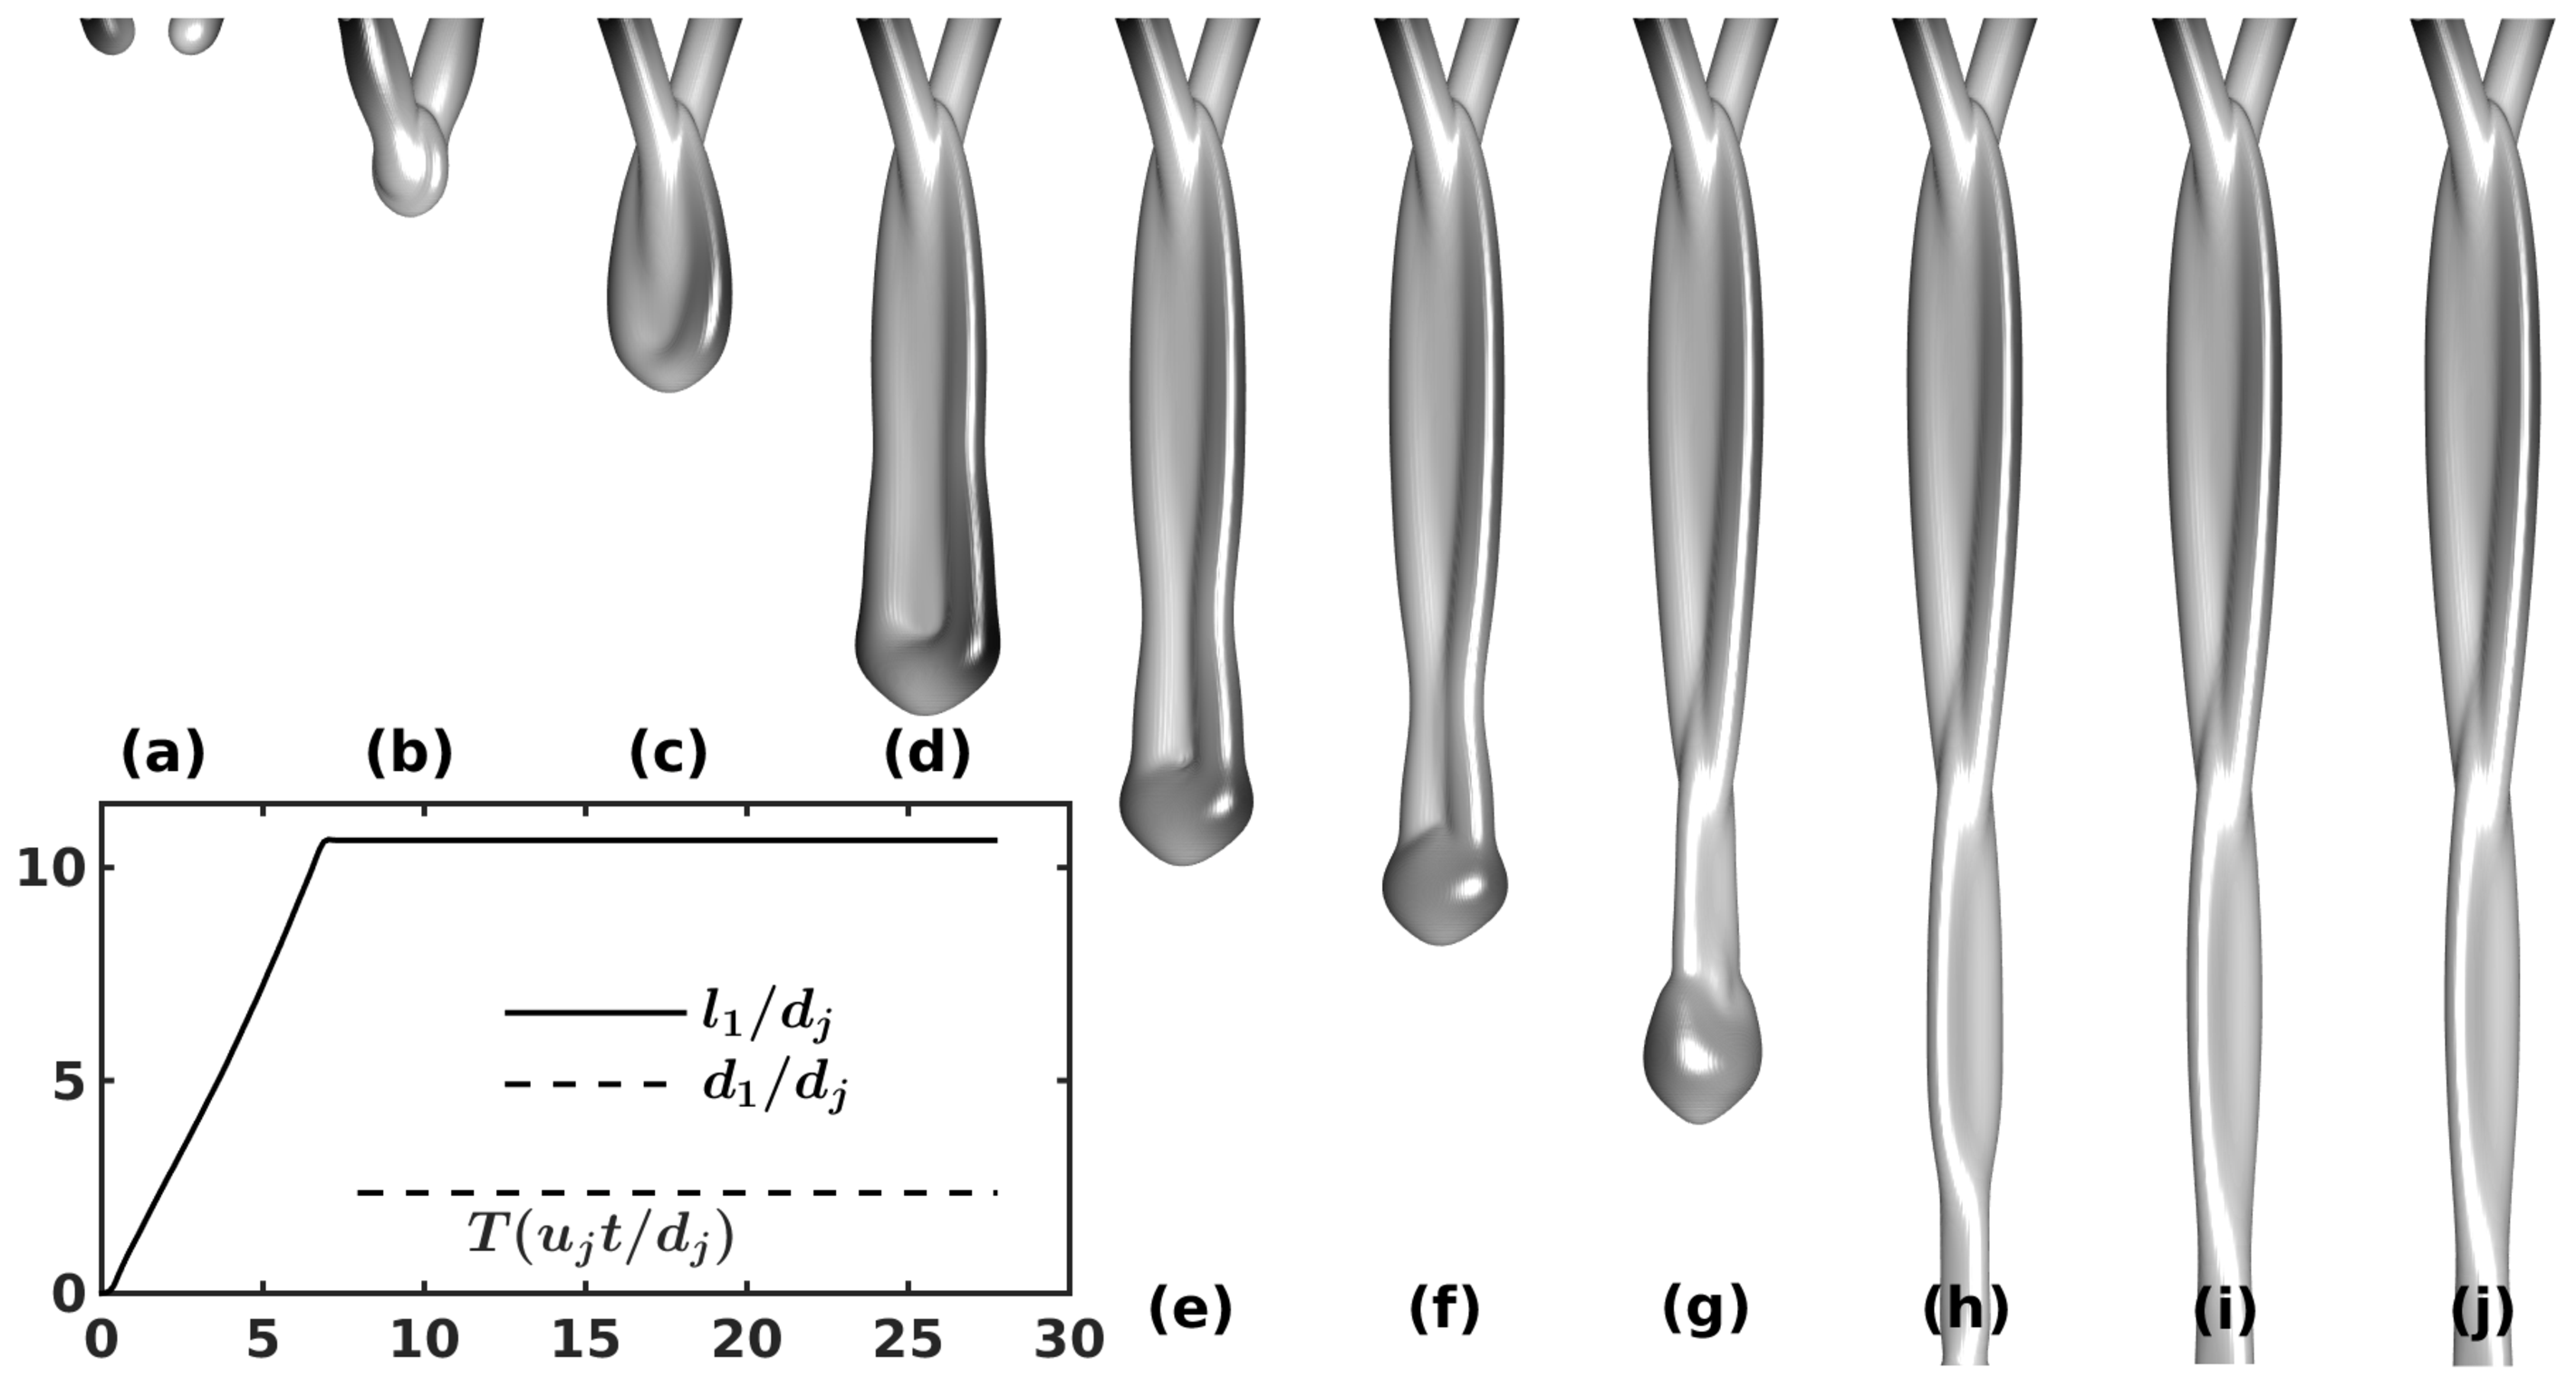
\includegraphics[width=\linewidth]{Figure3}
	\caption{Transition to the steady state fluid-links chain formed by collision of laminar jets. The figure illustrates the transient period through the temporal advancement from (a) pre-collision symmetric jets to $T (\frac{u_jt}{d_j}) = $ (b) 1.5, (c) 4, (d) 5, (e) 5.5, (f) 6.5, (g) 8.5, (h) 16.5, (i) and (j) 20}
	\label{Figure::transient}
\end{figure}
\clearpage
\begin{figure}
	\centering
	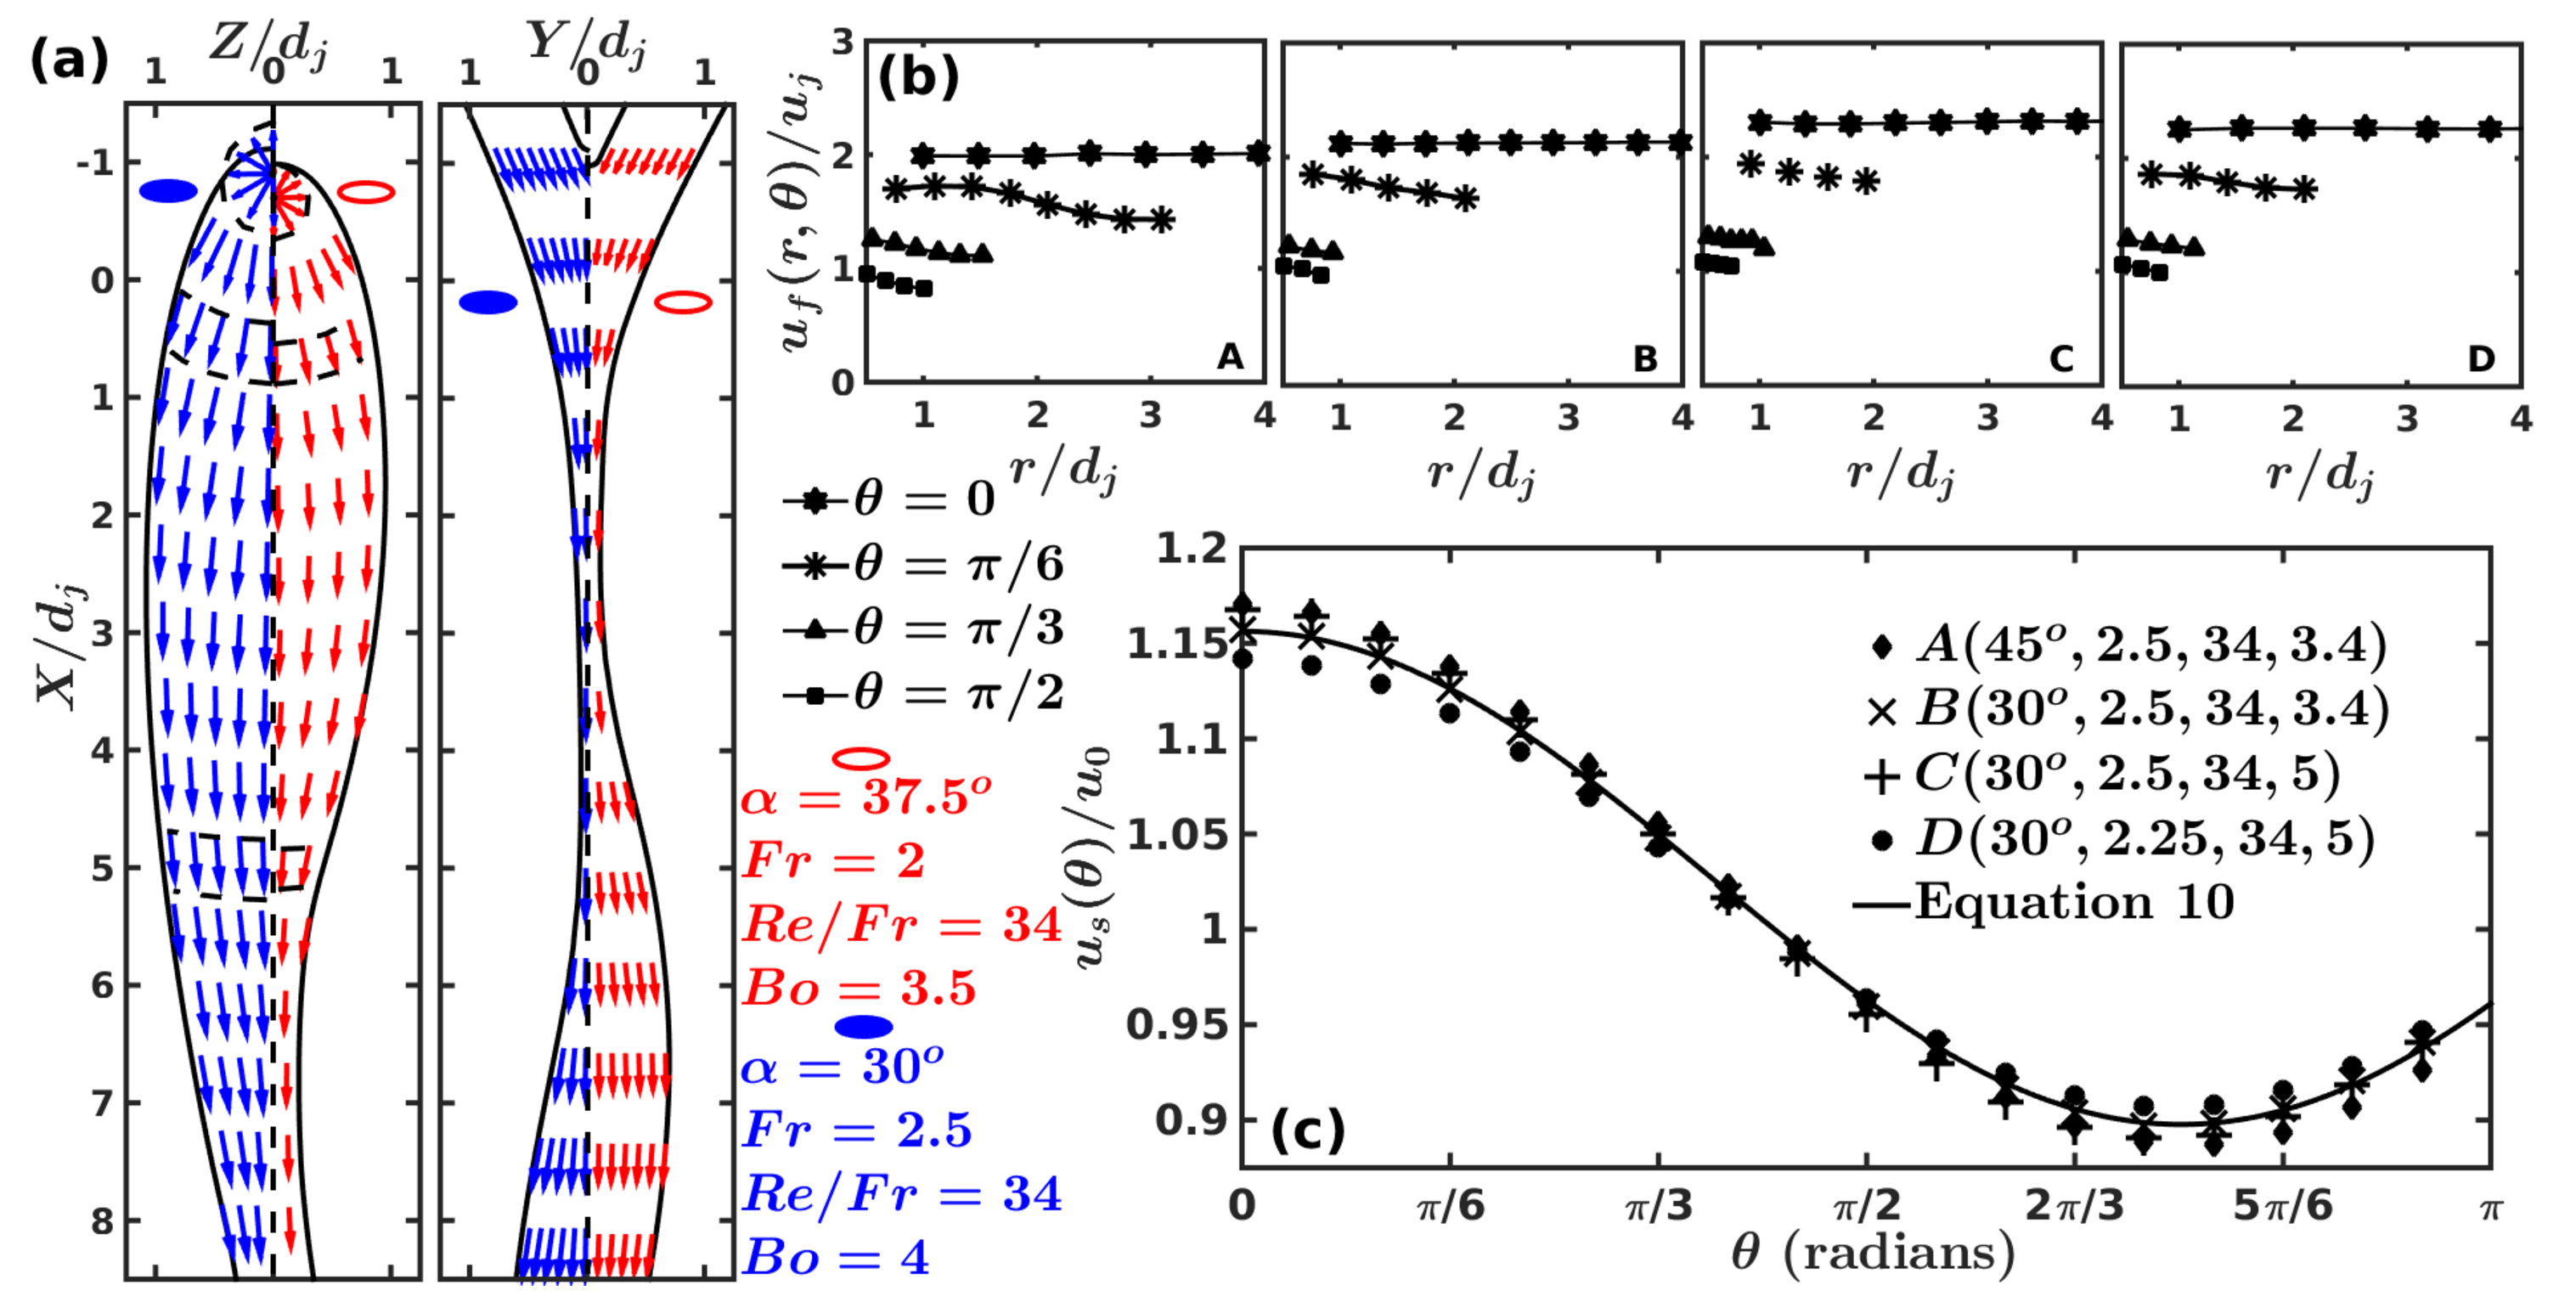
\includegraphics[width=\linewidth]{Figure4}
	\caption{Flow kinematics of the fluid parcels inside the liquid sheet: (a) Velocity vector field for two representative cases with different flow and physical parameters, the vector field is radial near the stagnation point and then follows the self similar phase contour, (b) Variation of velocity in the radial direction for four representative cases with ($\alpha$, $Fr$, $Re/Fr$, $Bo$): A(45$\degree$, 2.5, 34, 3.4), B(30$\degree$, 2.5, 34, 3.4), C(30$\degree$, 2.5, 34, 5) and D(30$\degree$, 2.25, 34, 5) and (c) Variation of the radially averaged sheet velocity ($u_s$), non-dimensionalized with the average sheet velocity ($u_0$) along the azimuthal direction in the sheet.}
	\label{Figure::velocityVectors}
\end{figure}
\clearpage
\begin{figure}
	\centering
	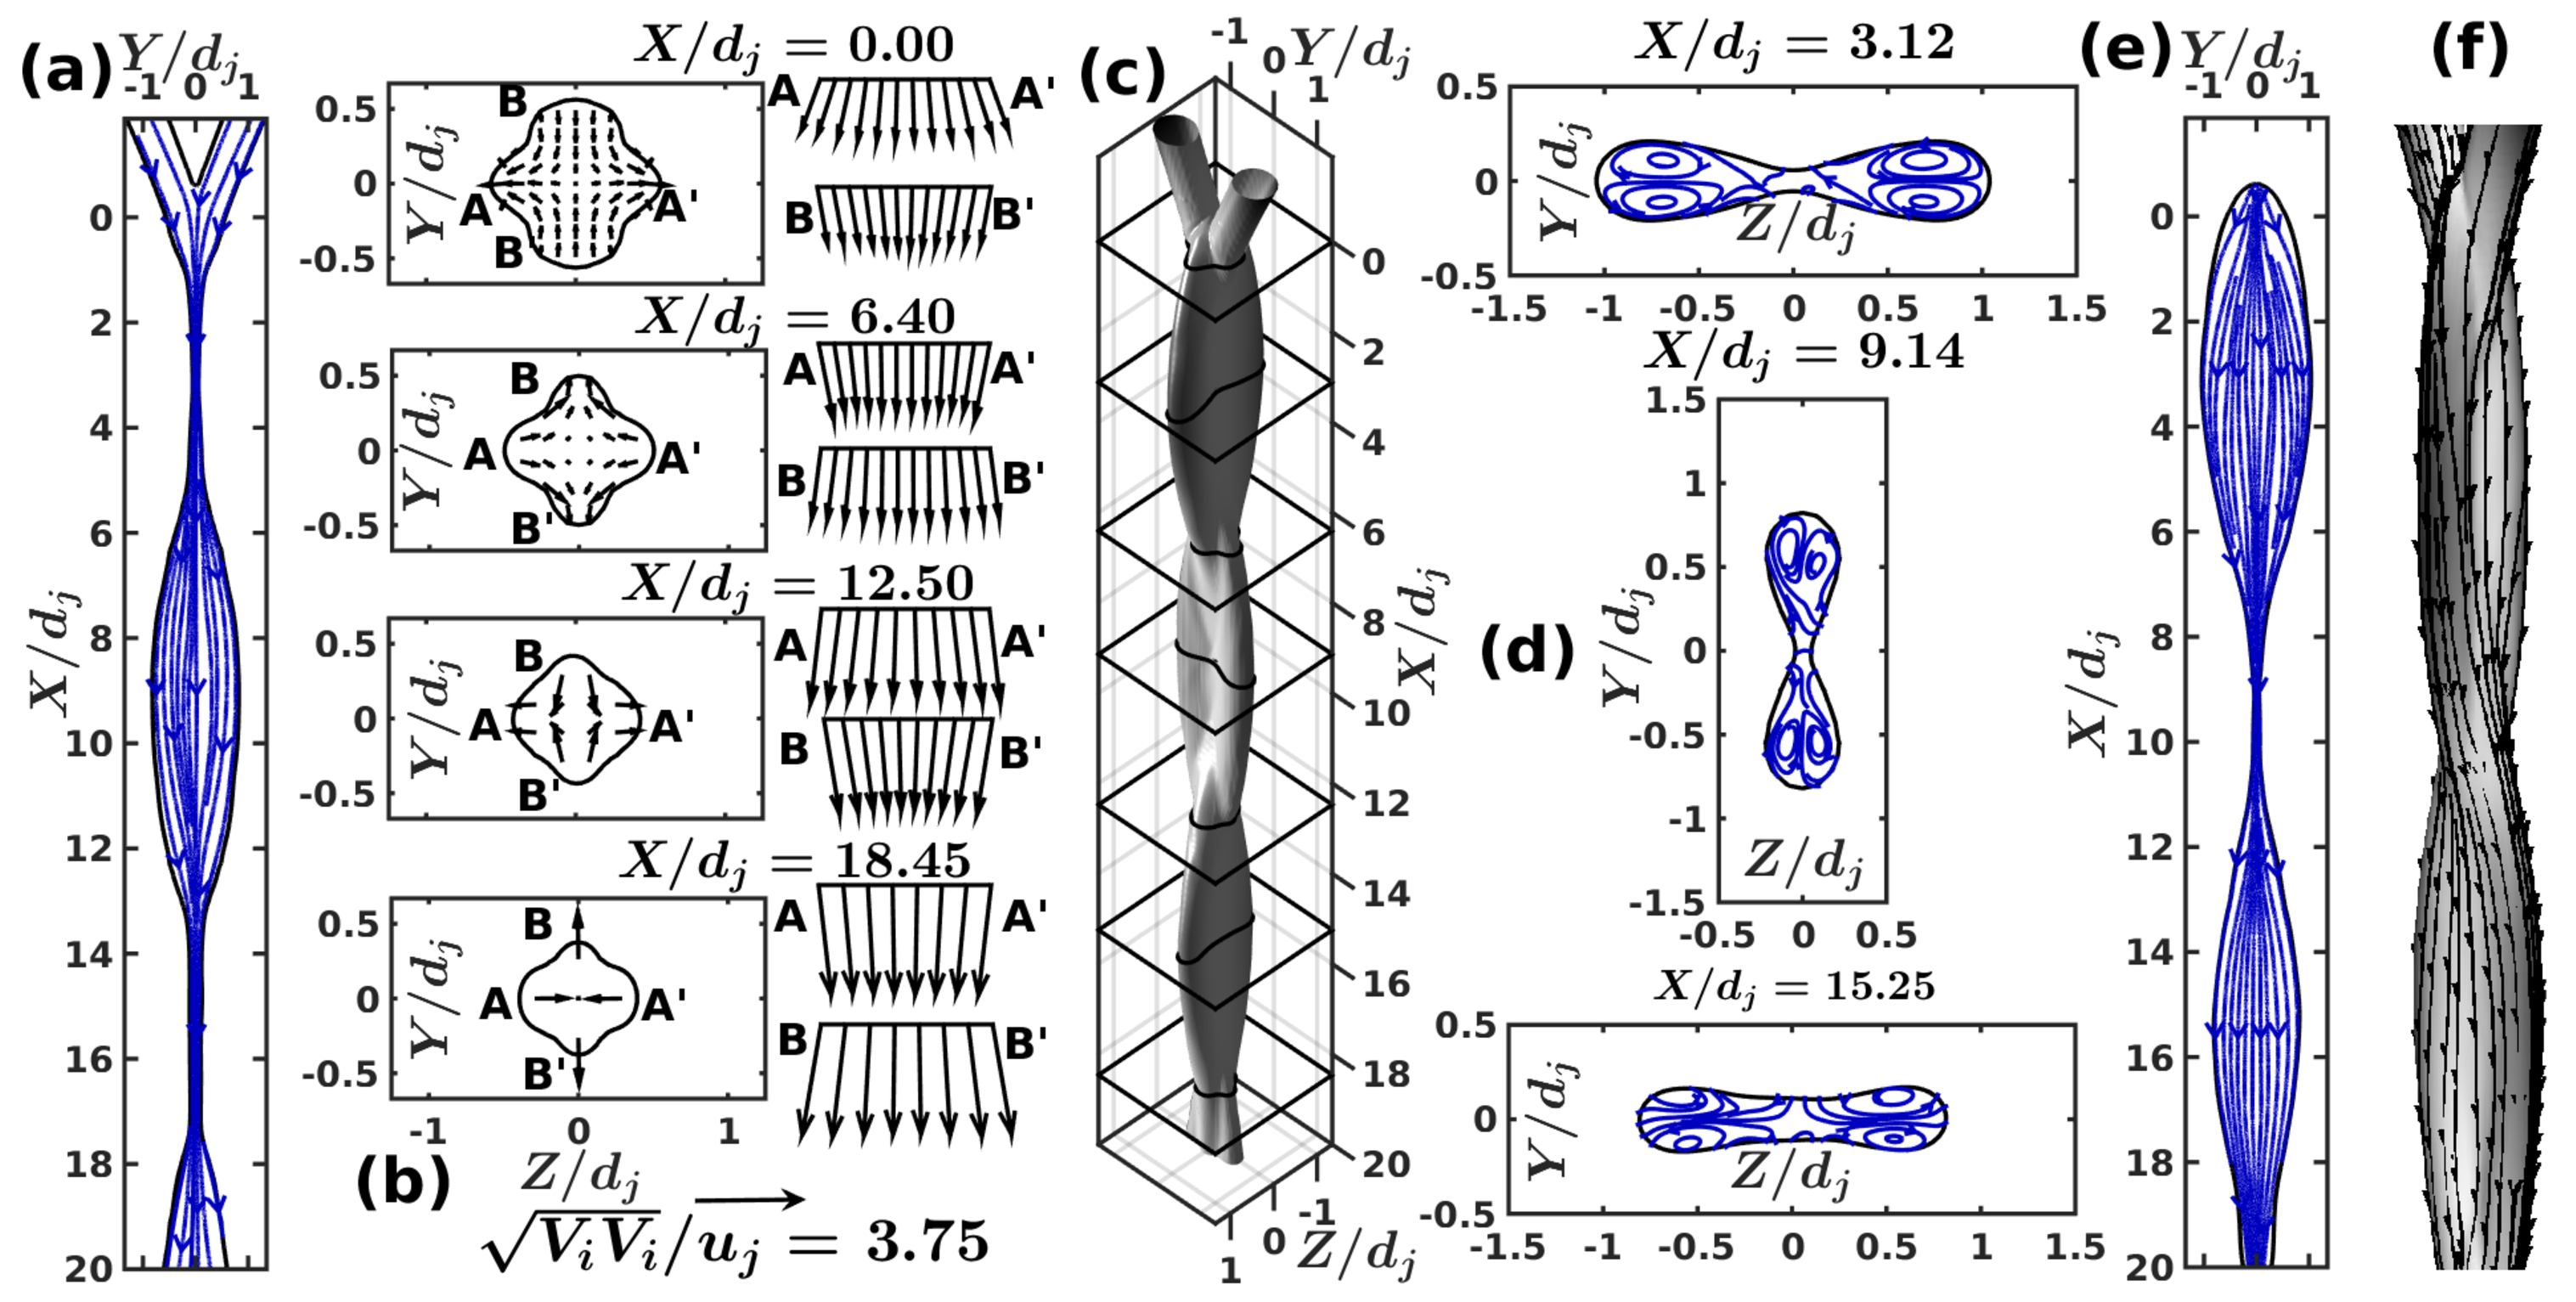
\includegraphics[width=\linewidth]{Figure5}
	\caption{Flow kinematics of the fluid parcels inside the liquid sheet: (a) Velocity vector field for two representative cases with different flow and physical parameters, the vector field is radial near the stagnation point and then follows the self similar phase contour, (b) Variation of velocity in the radial direction for four representative cases with ($\alpha$, $Fr$, $Re/Fr$, $Bo$): A(45$\degree$, 2.5, 34, 3.4), B(30$\degree$, 2.5, 34, 3.4), C(30$\degree$, 2.5, 34, 5) and D(30$\degree$, 2.25, 34, 5) and (c) Variation of the radially averaged sheet velocity ($u_s$), non-dimensionalized with the average sheet velocity ($u_0$) along the azimuthal direction in the sheet.}
	\label{Figure::streamDetails}
\end{figure}
\clearpage
\begin{figure}
	\centering
	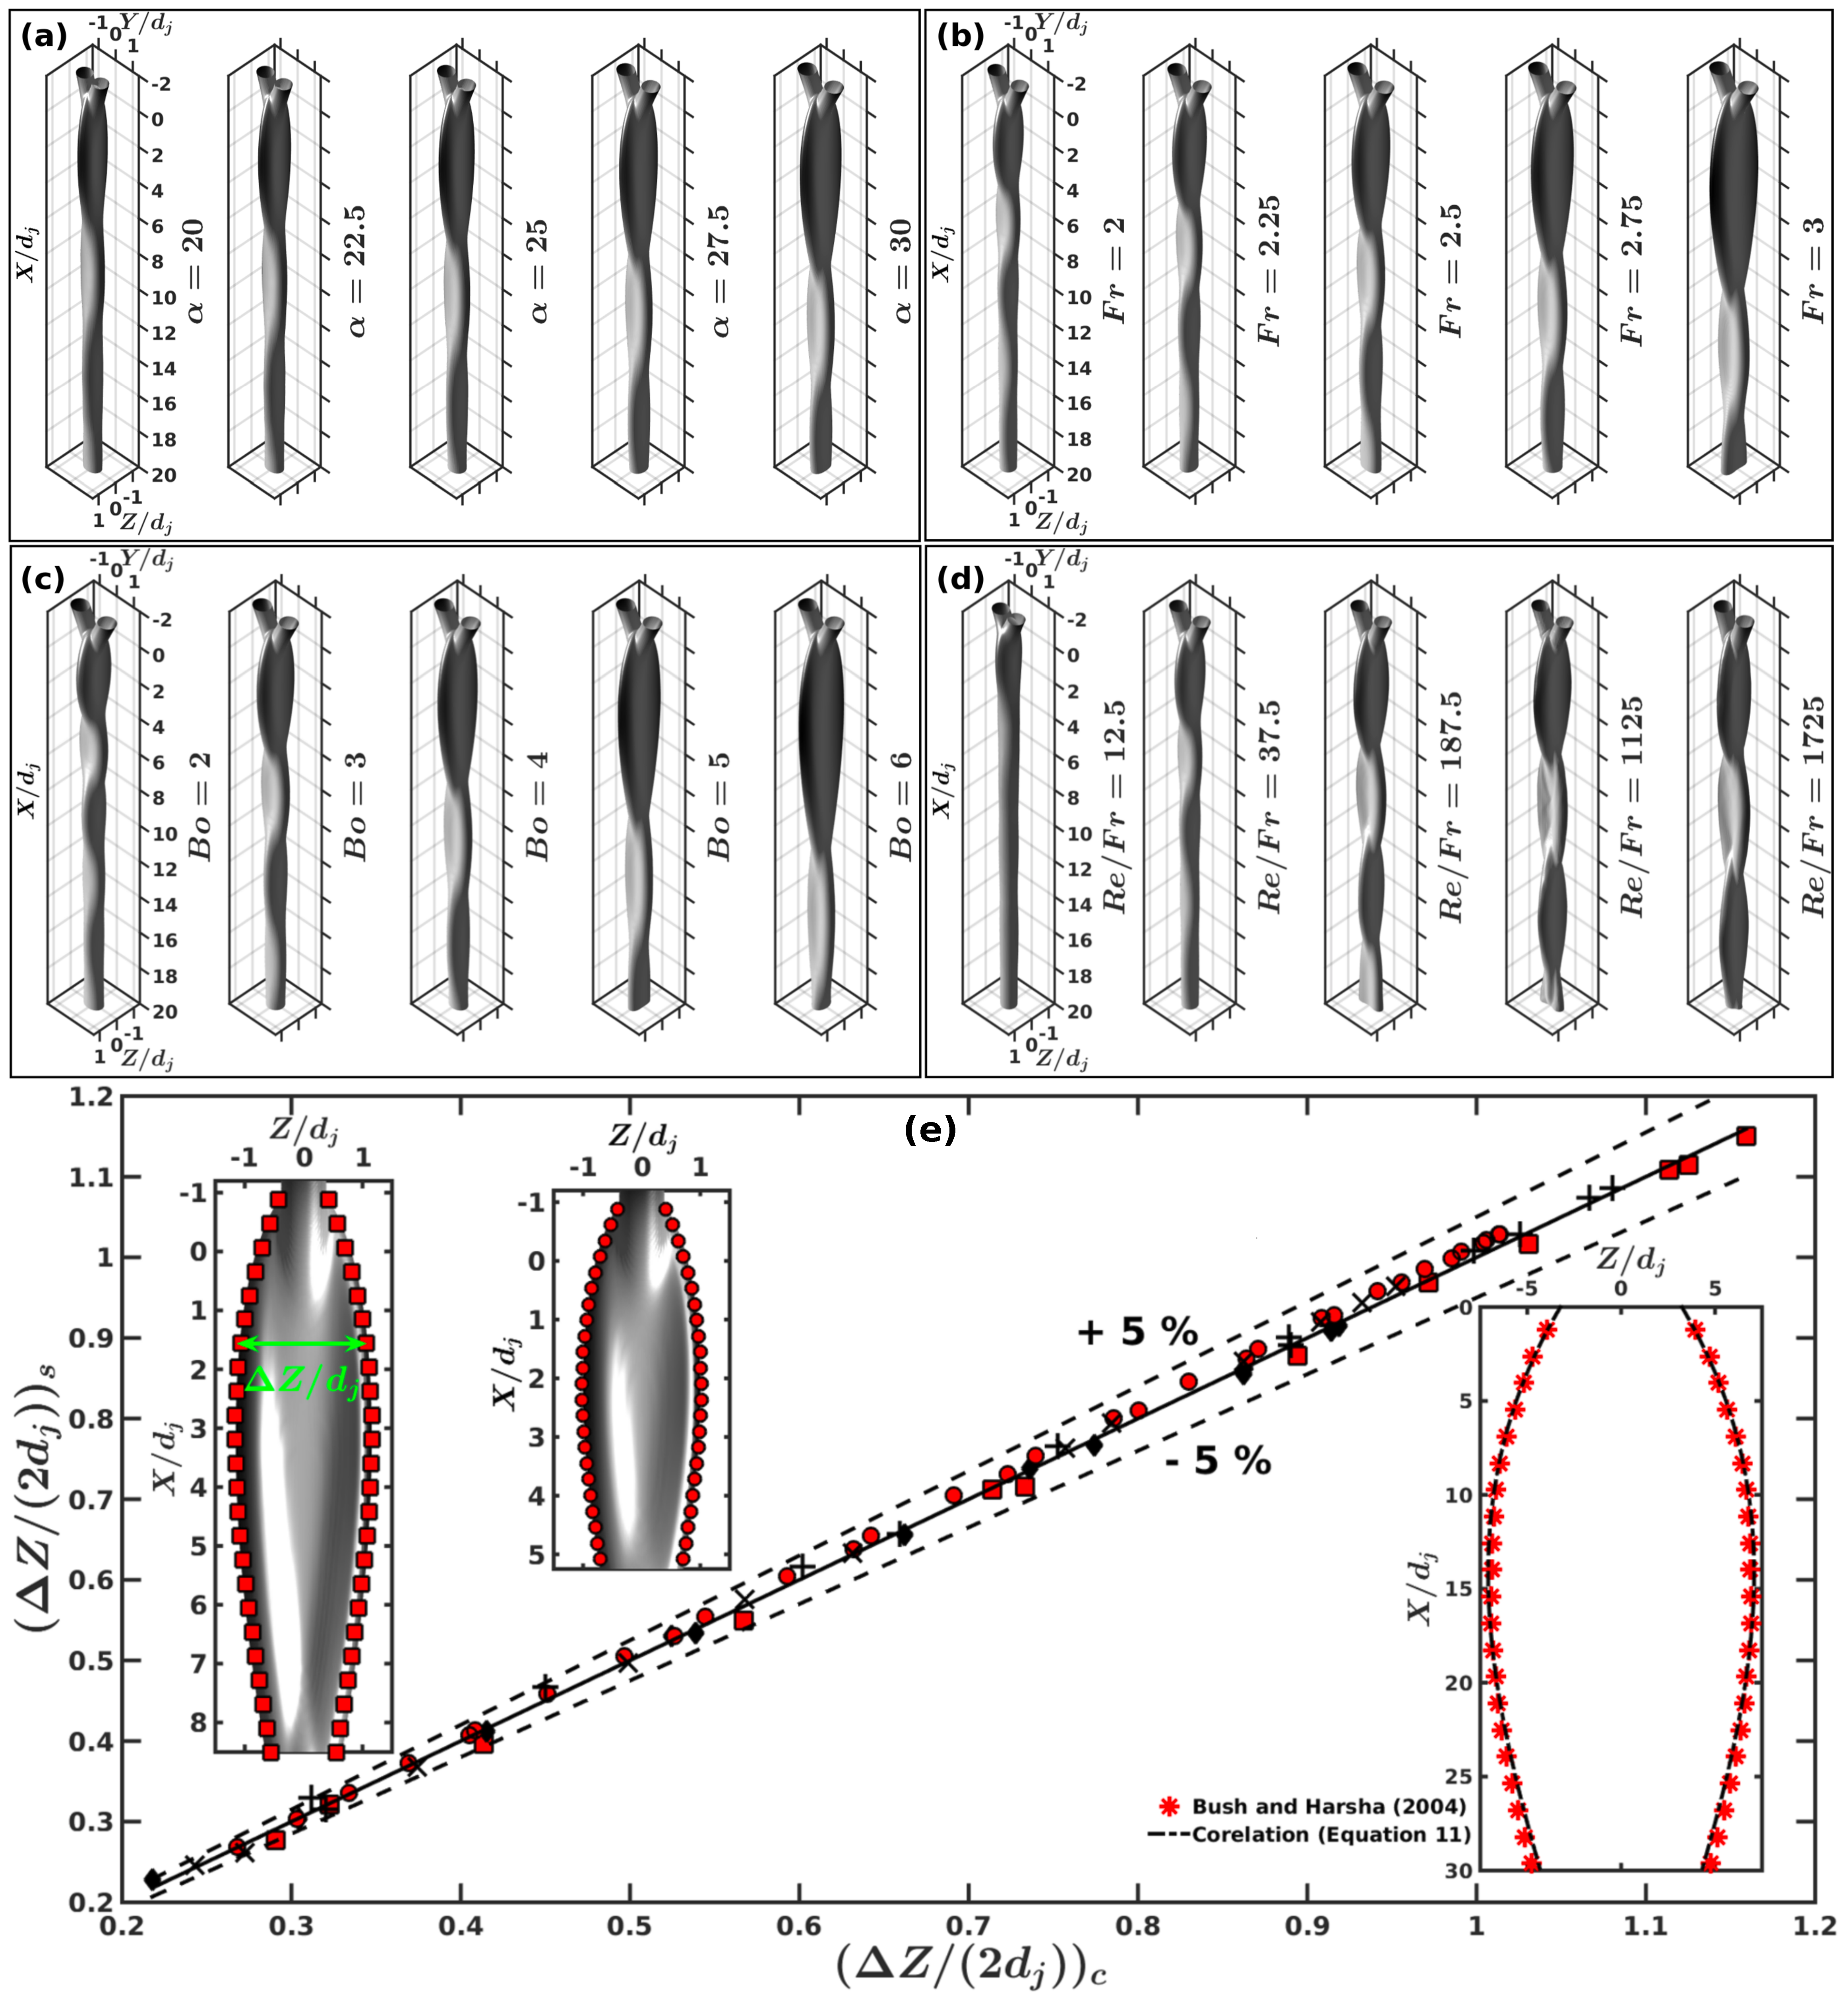
\includegraphics[width=\linewidth]{Figure6}
	\caption{High fidelity numerical simulations of liquid jets collision to form chain structure for variation of (a) $Re/Fr$ at $Fr$ = 2,$Bo$ = 3.4, $\alpha$ = 30 (b) $Fr$ at $Re/Fr$ = 34,$Bo$ = 3.4, $\alpha$ =  30 (c) $Bo$ at $Re/Fr$ = 34,$Fr$ = 2.5, $\alpha$ = 30 and (d) $\alpha$ at $Re/Fr$ = 34,$Fr$ = 2.5, $Bo$ = 4.57}
	\label{Figure::phaseContours}
\end{figure}
\clearpage
\begin{table}
	\centering
	\begin{tabular}{@{}cccccc@{}}
		&$C_0$ & $C_1$ & $C_2$ & $C_3$ & $C_4$    \\ 
		$p_0$&3.662&-0.082&-2.822&-1.504&-0.657\\
		$p_1$&2.720&~0.490&-1.231&-0.831&-0.290\\
		$p_2$&0.353&~1.146&~0.437&~0.074&~0.029\\
		$p_3$&0.512&~0.592&~0.800&-0.065&~0.039\\ 
	\end{tabular}
\caption{Factors ($C_{m,n}$) involved in Equation~\ref{Equation::CorelationCoefficeints} determined by regression analysis to get the coefficients $p_n$ of Equation~\ref{Equation::correlation}}
\label{Table::CorrelationPrams}
\end{table}
\begin{figure}
	\centering
	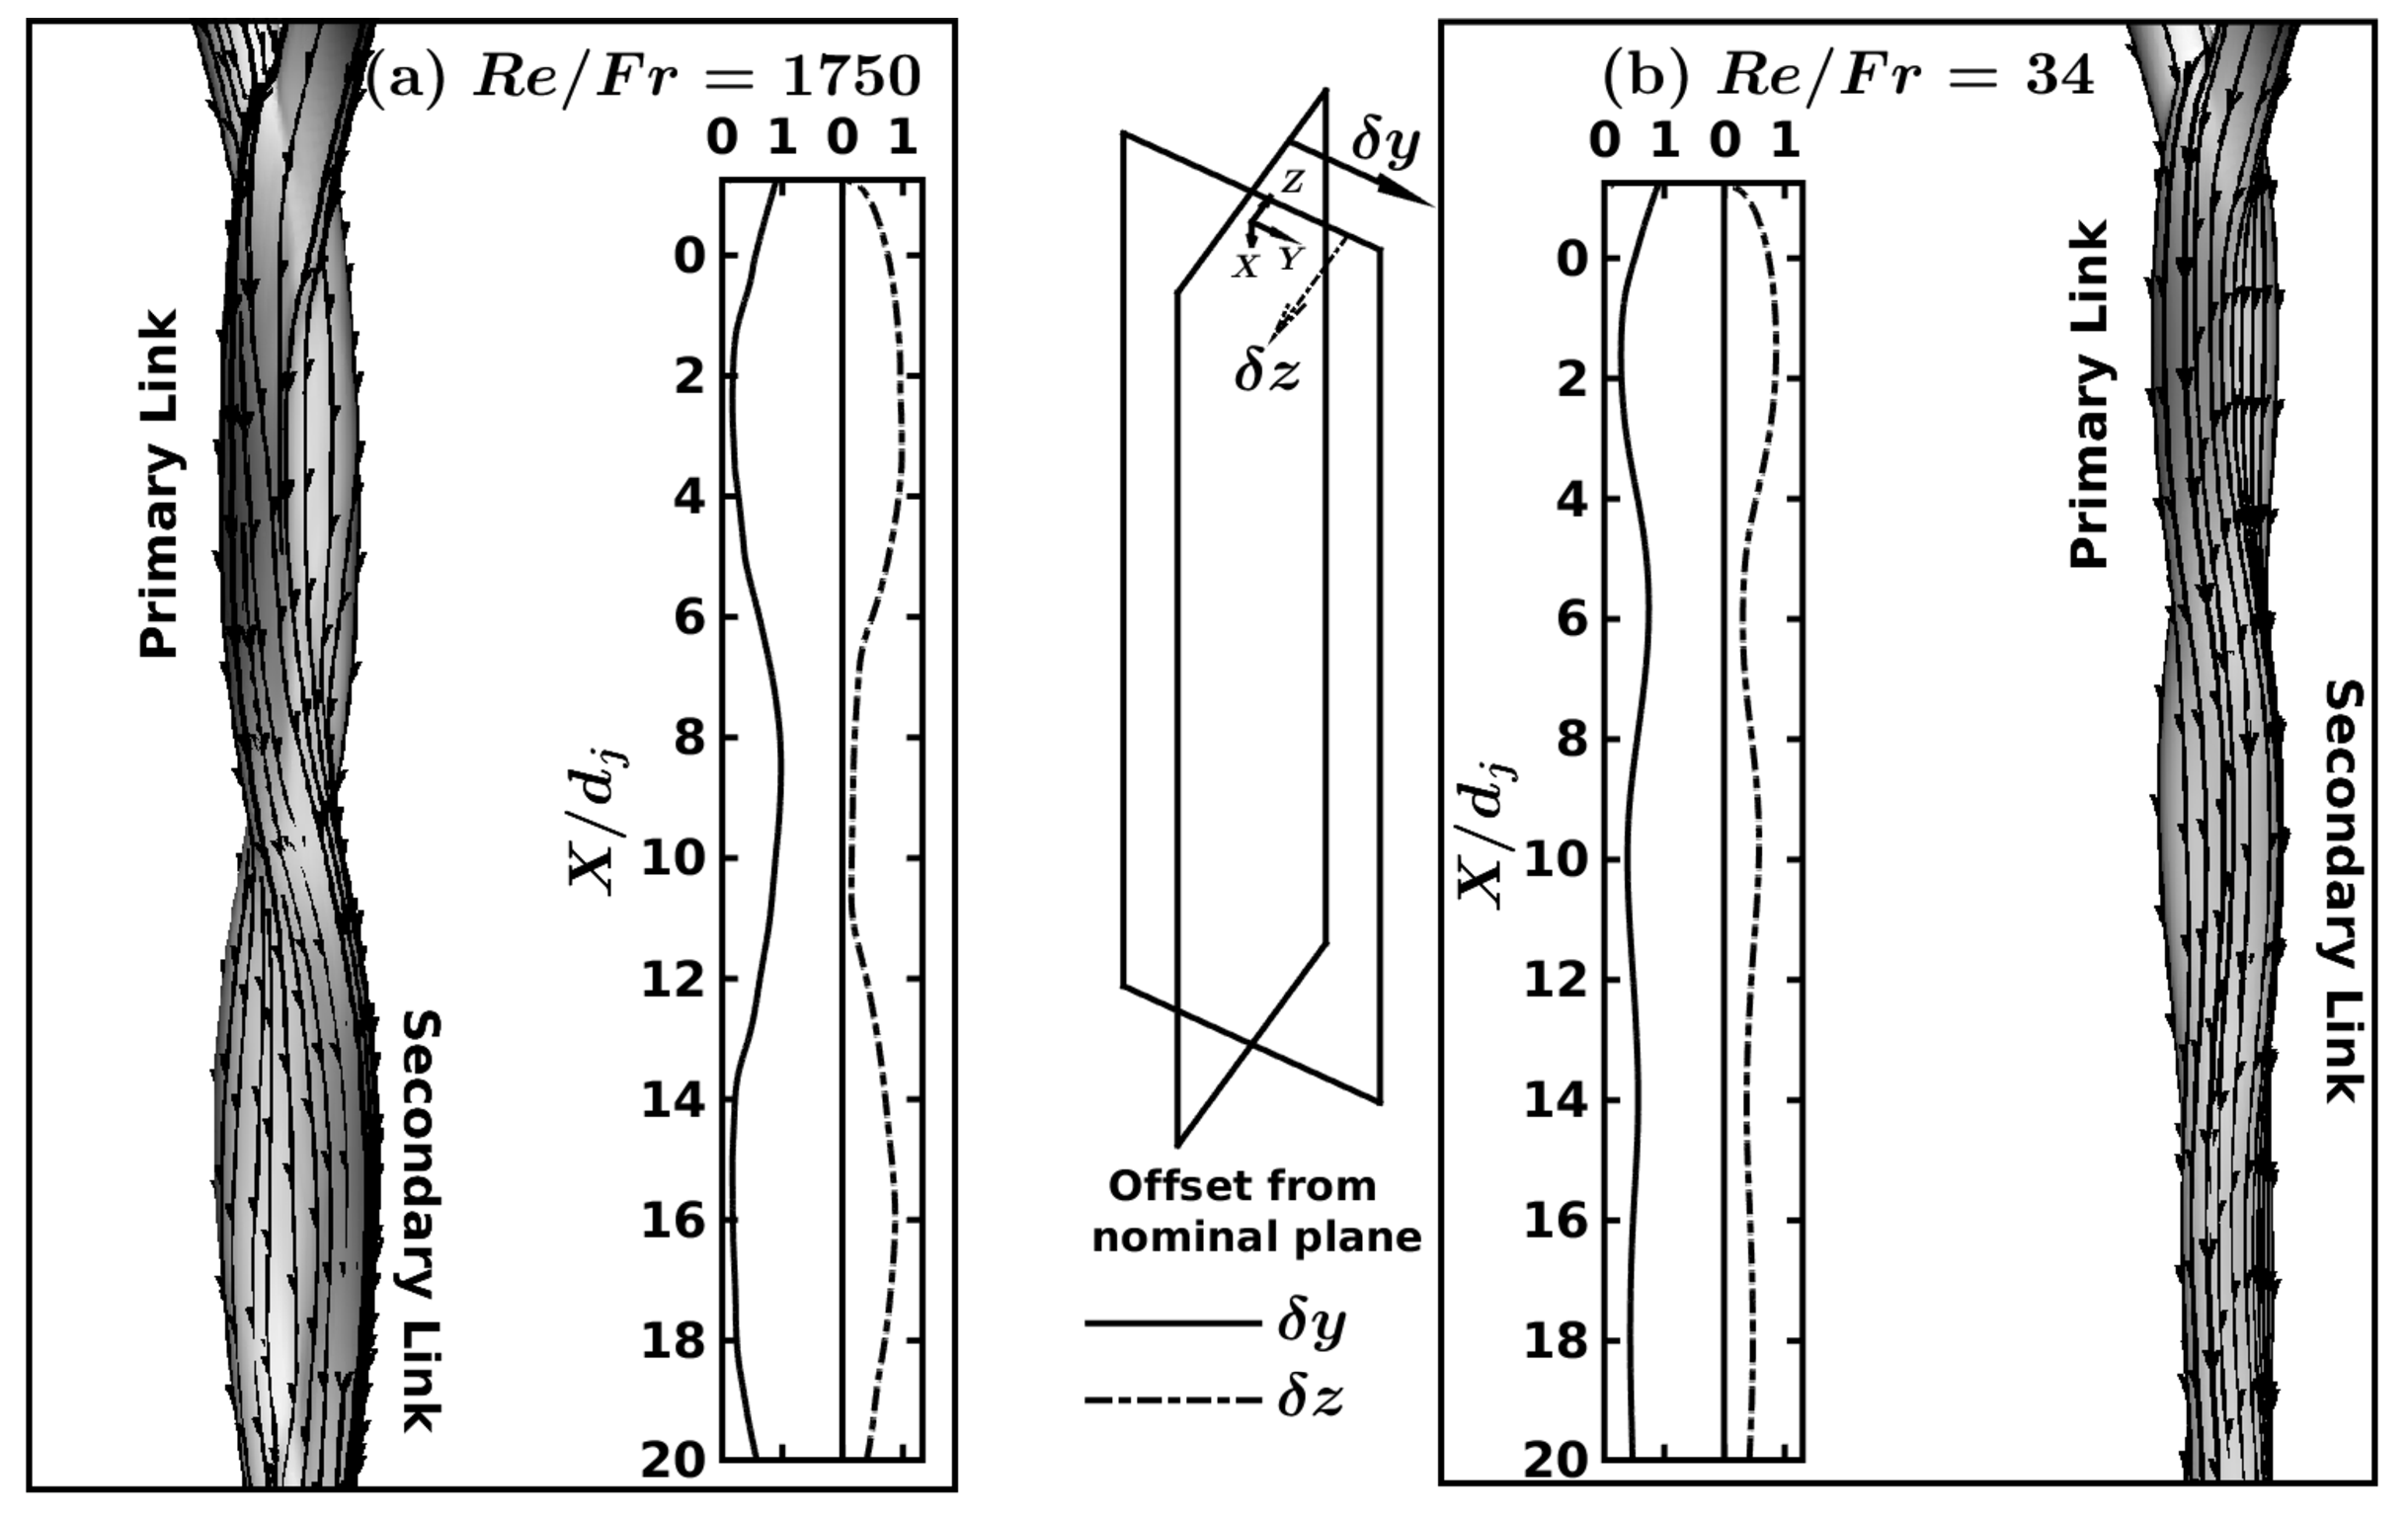
\includegraphics[width=\linewidth]{Figure7}
	\caption{Comparison between the values of expansion of the sheet outer periphery $\left(\Delta Z(x)\right)$ as obtained from correlations $\left((\Delta Z/(2d_j))_c\right)$ given in Equation~\ref{Equation::correlation} and from numerical simulations $\left((\Delta Z/(2d_j))_s\right)$ for different parametric variations of testing data with (symbol, $\alpha$, $Fr$, $Re/Fr$, $Bo$) = (\protect\MarkerSquareRed, 30$\degree$, 2.5, 34, 5): first inset figure from the left; (+, 30$\degree$, 2.5, 34, 4); (\protect \MarkerDiamondBlack, 30$\degree$, 2.5, 20, 2.3); ($\times$, 25$\degree$, 2.5, 34, 4.57) and (\protect \MarkerCircleRed, 30$\degree$, 2.5, 20, 3.75): second inset figure from the left. In the last inset figure (from the left), comparison between the  correlation model given in Equation~\ref{Equation::correlation} and experimental results of \cite{bush2004collision} is provided.}
	\label{Figure::corelatehx}
\end{figure}
\clearpage
\begin{figure}
	\centering
	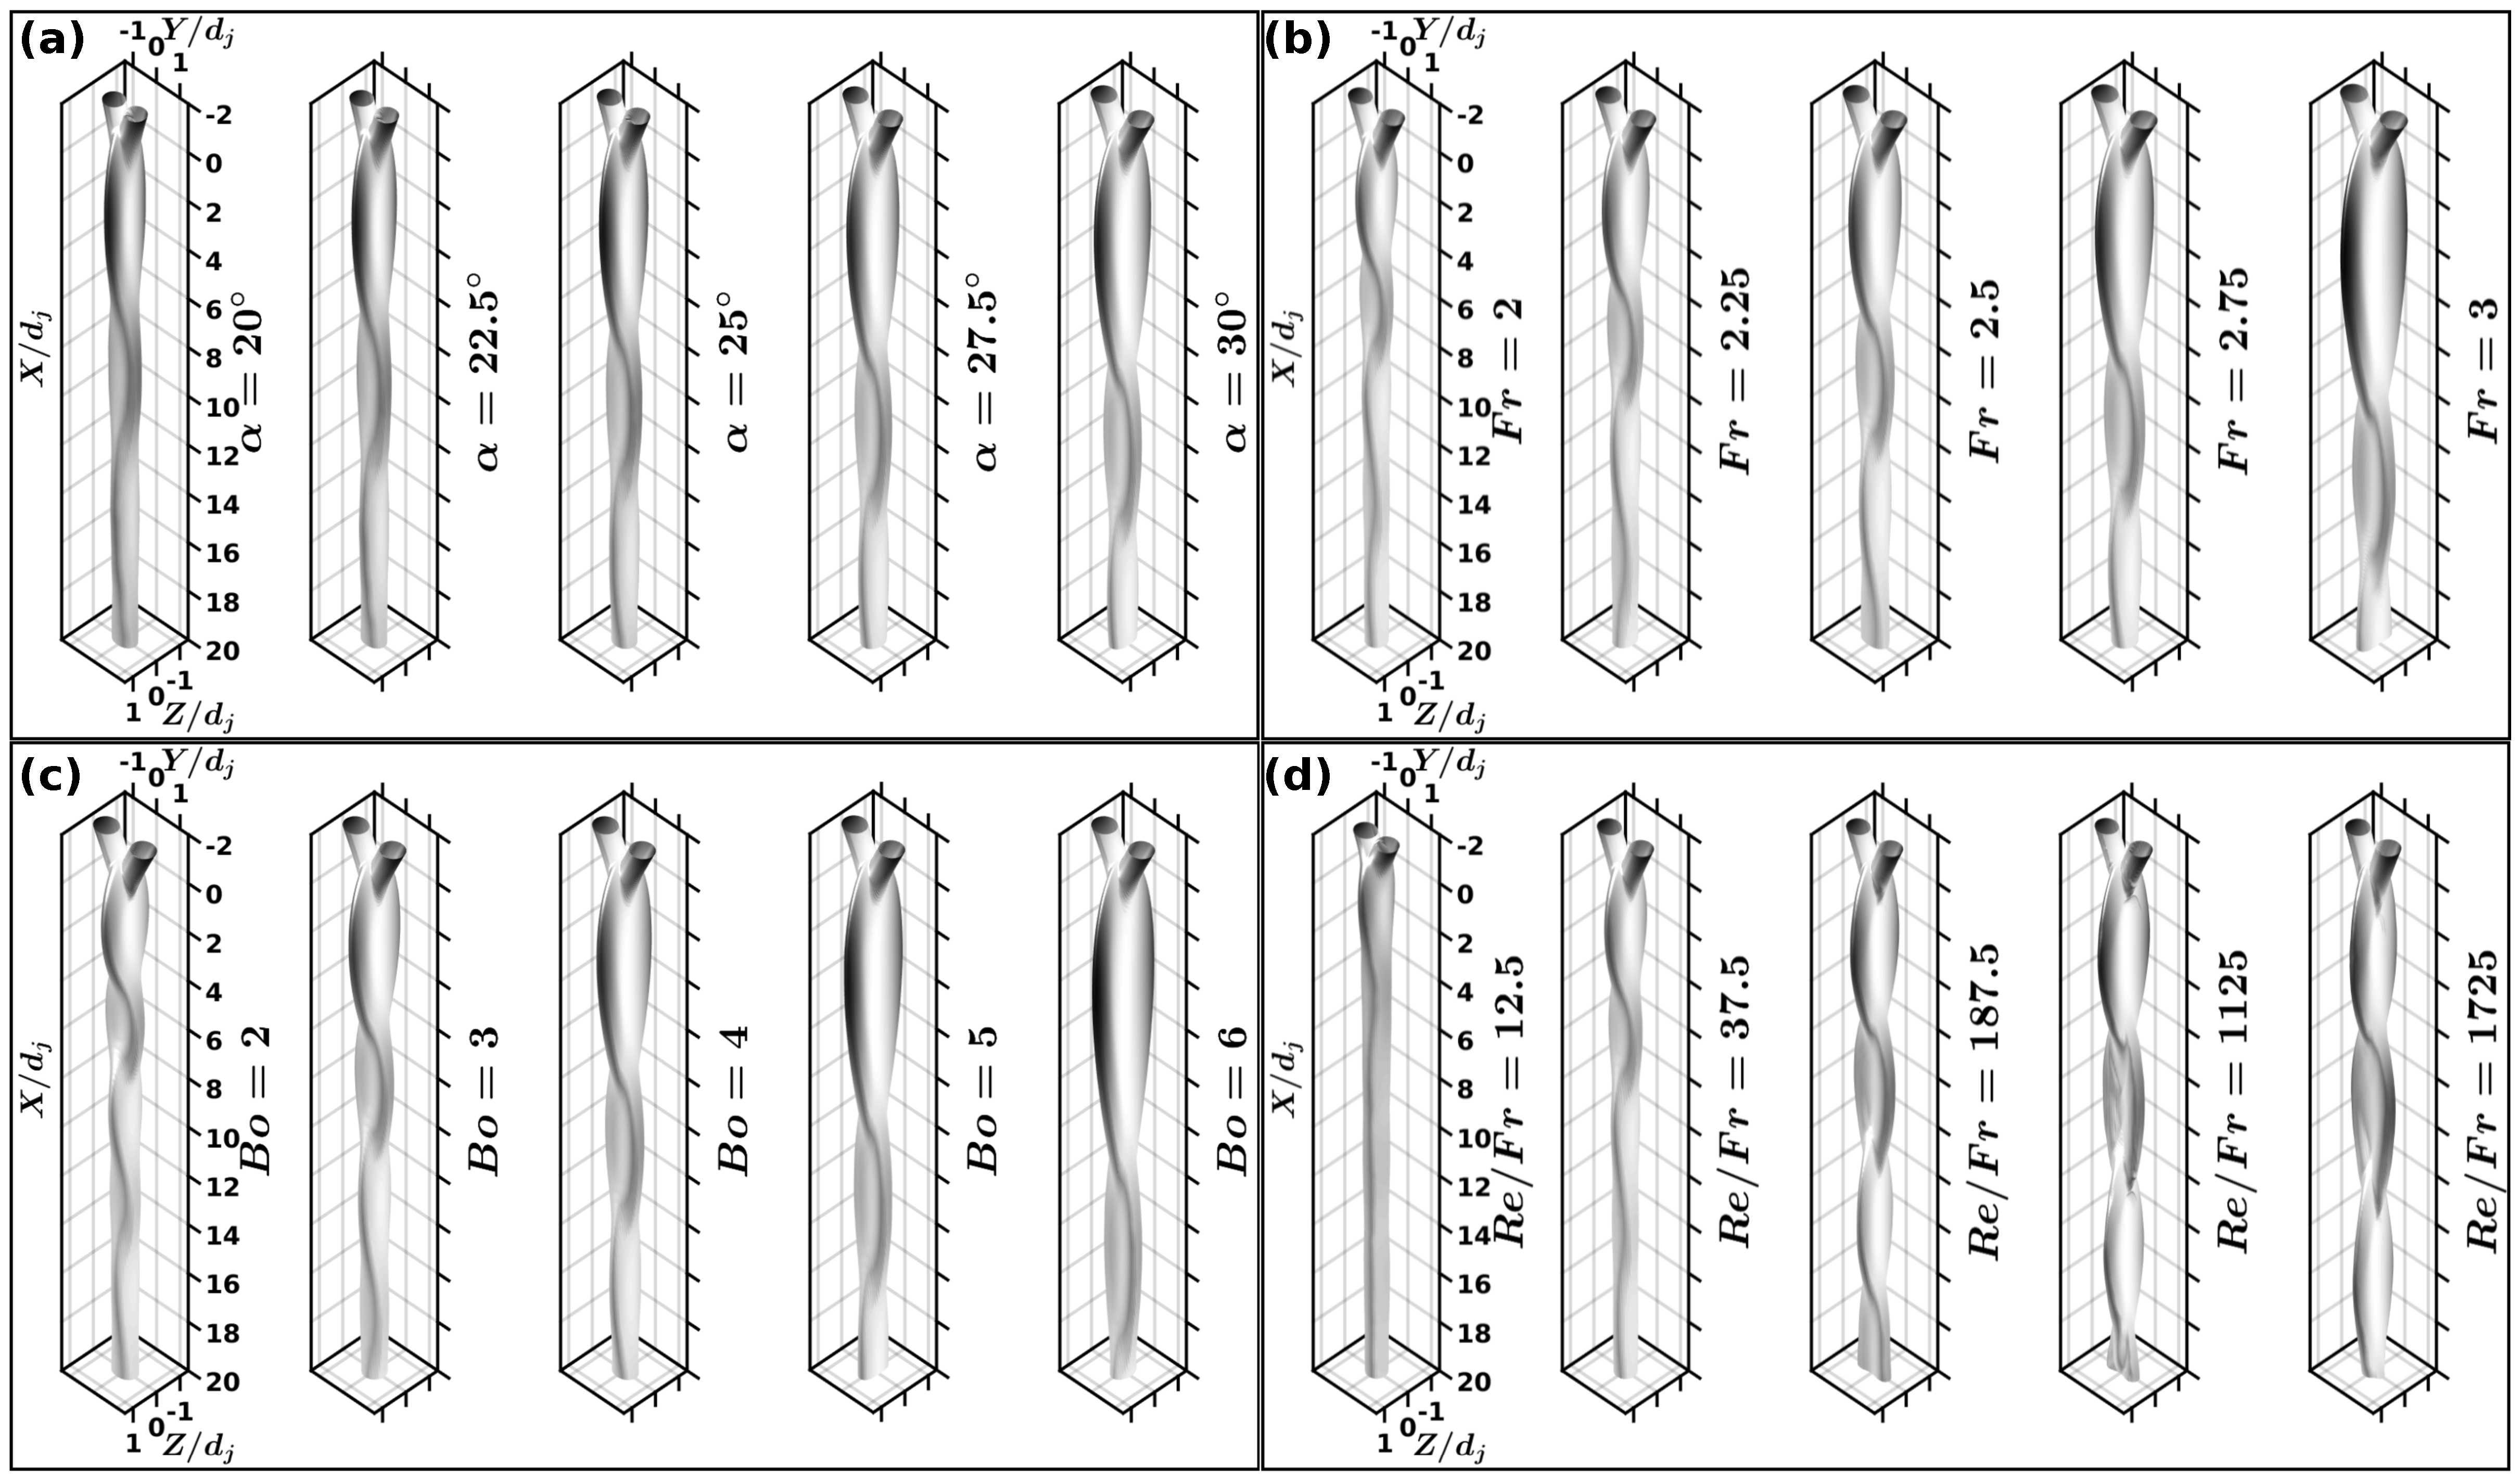
\includegraphics[width=\linewidth]{Figure8}
	\caption{Comparison between the link shape and dimension obtained through numerical simulations (iso-surface volume contours) and by using the analytical model using force balance (red colored symbols \protect\MarkerSquareRed) for different flow configurations ($\alpha$, $Fr$, $Re/Fr$, $Bo$, $\epsilon$): (a) (), (b) (), (d) () and (e) (), where $\epsilon$ is the $L^1$ relative error norm given by Equation~\ref{Equation::L1}. In Figure (c), the schematic of this analytical model is shown.}
	\label{Figure::analytical}
\end{figure}
\clearpage
\begin{figure}
	\centering
	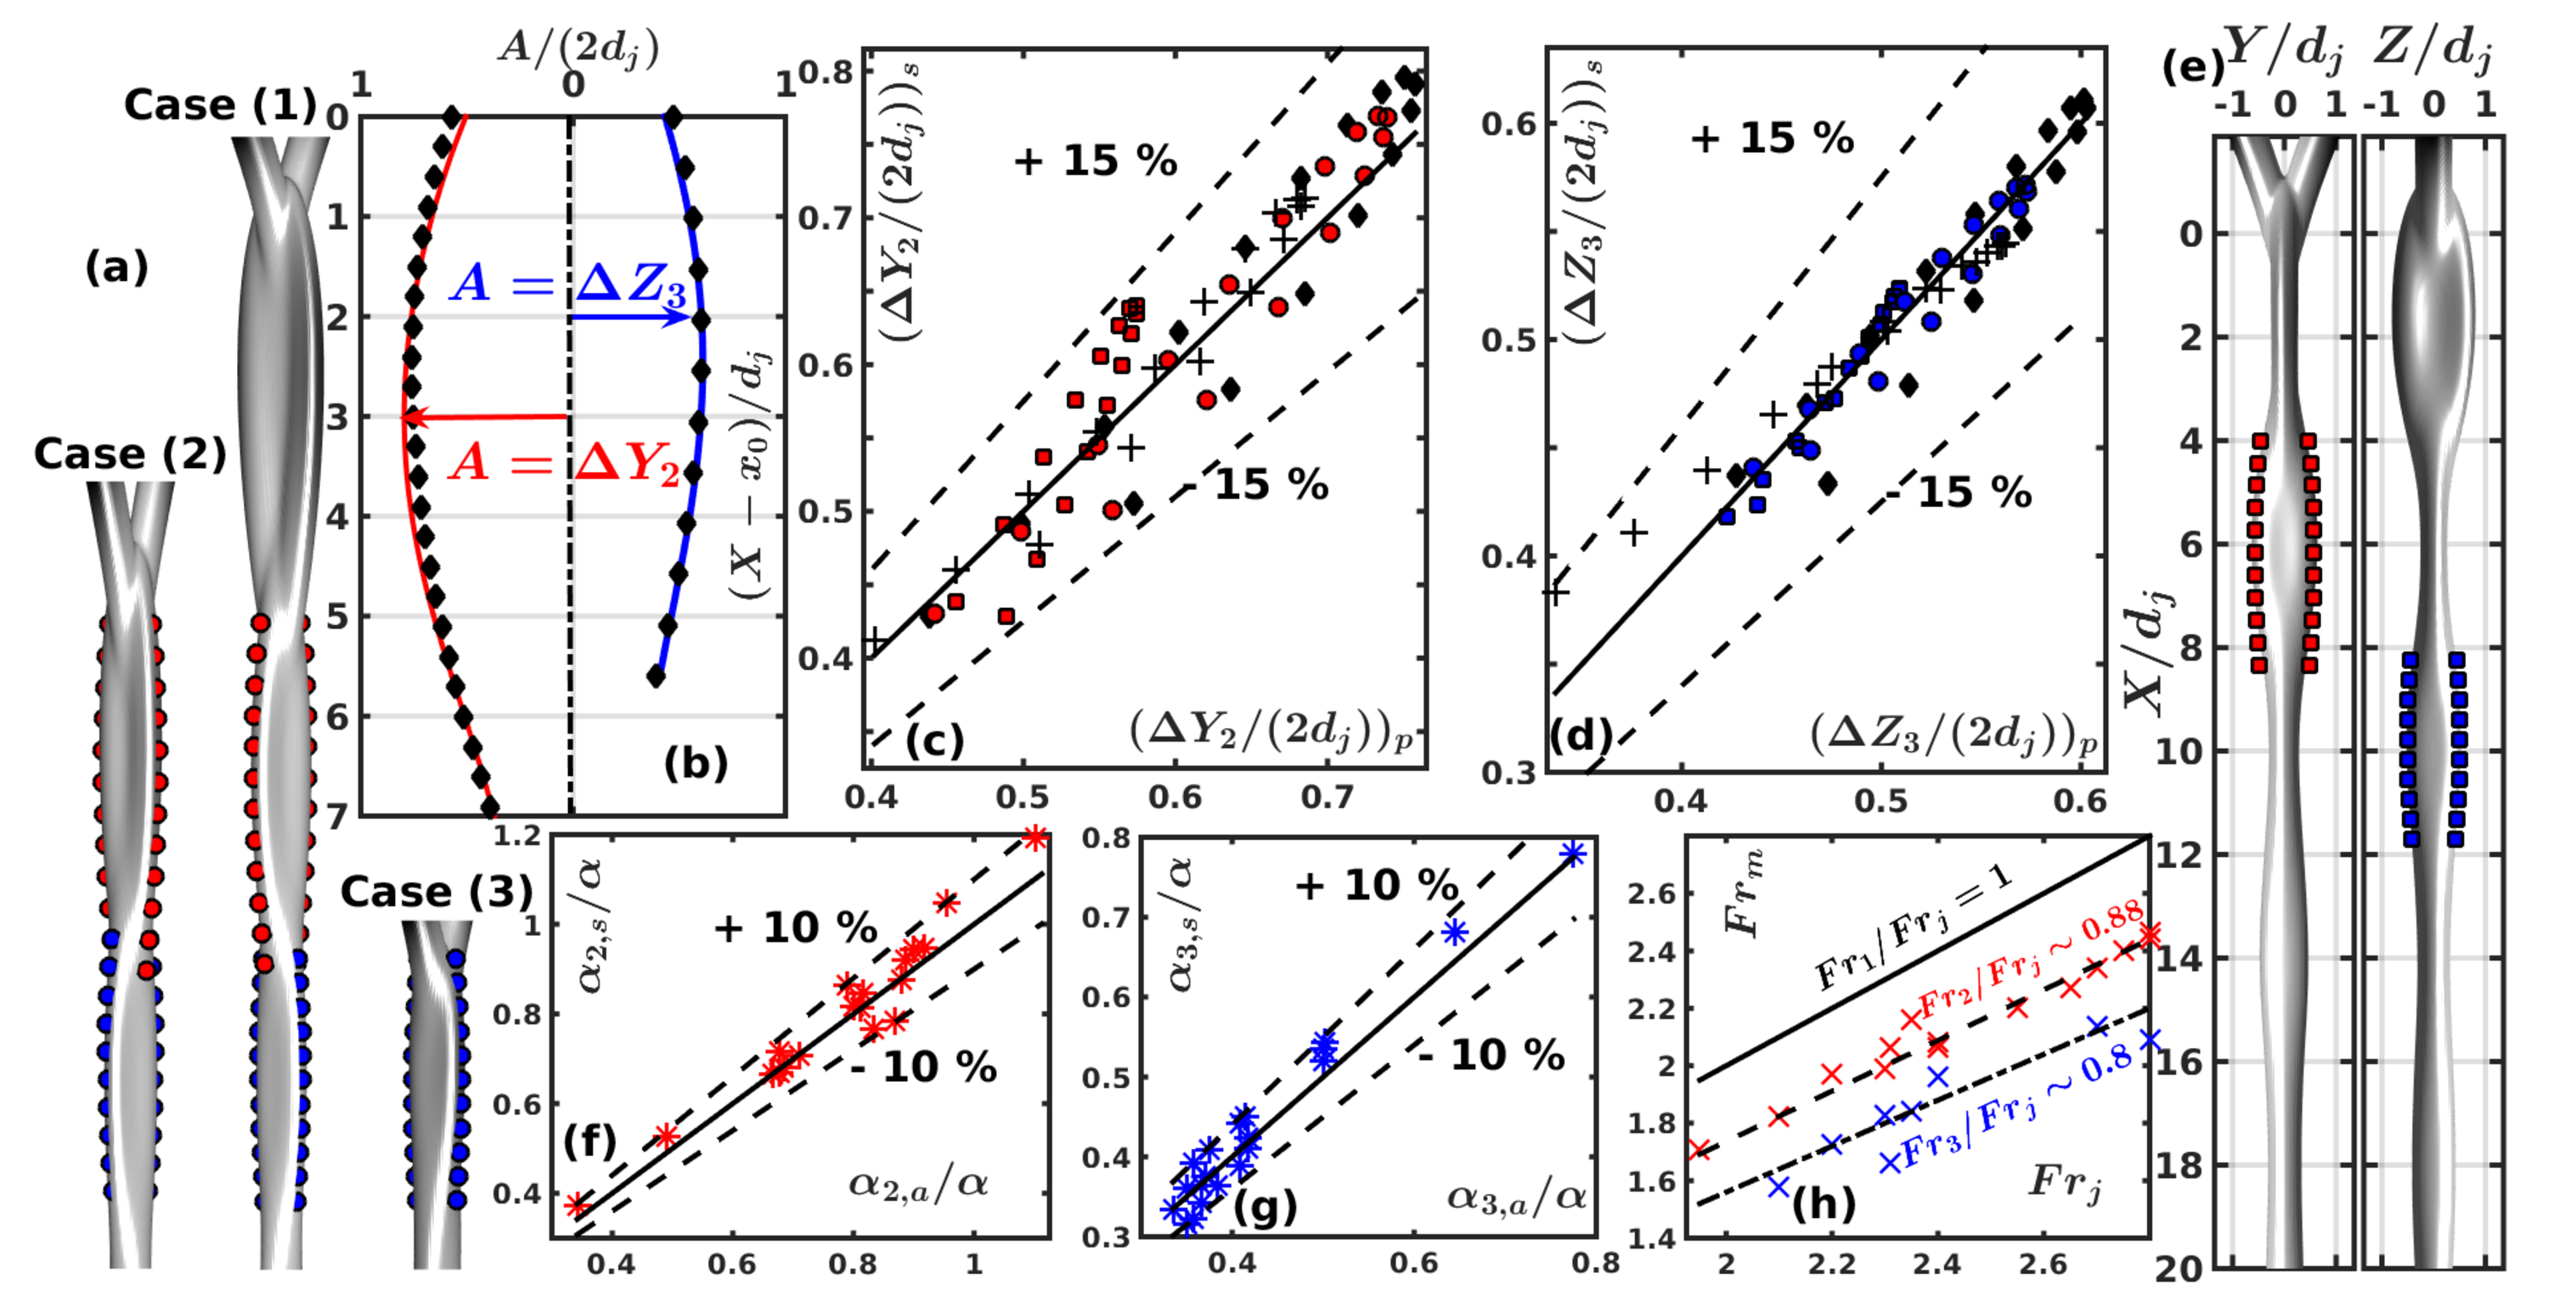
\includegraphics[width=\linewidth]{Figure9}
	\caption{}
	\label{Figure::secondCollision}
\end{figure}
\clearpage
\begin{figure}
	\centering
	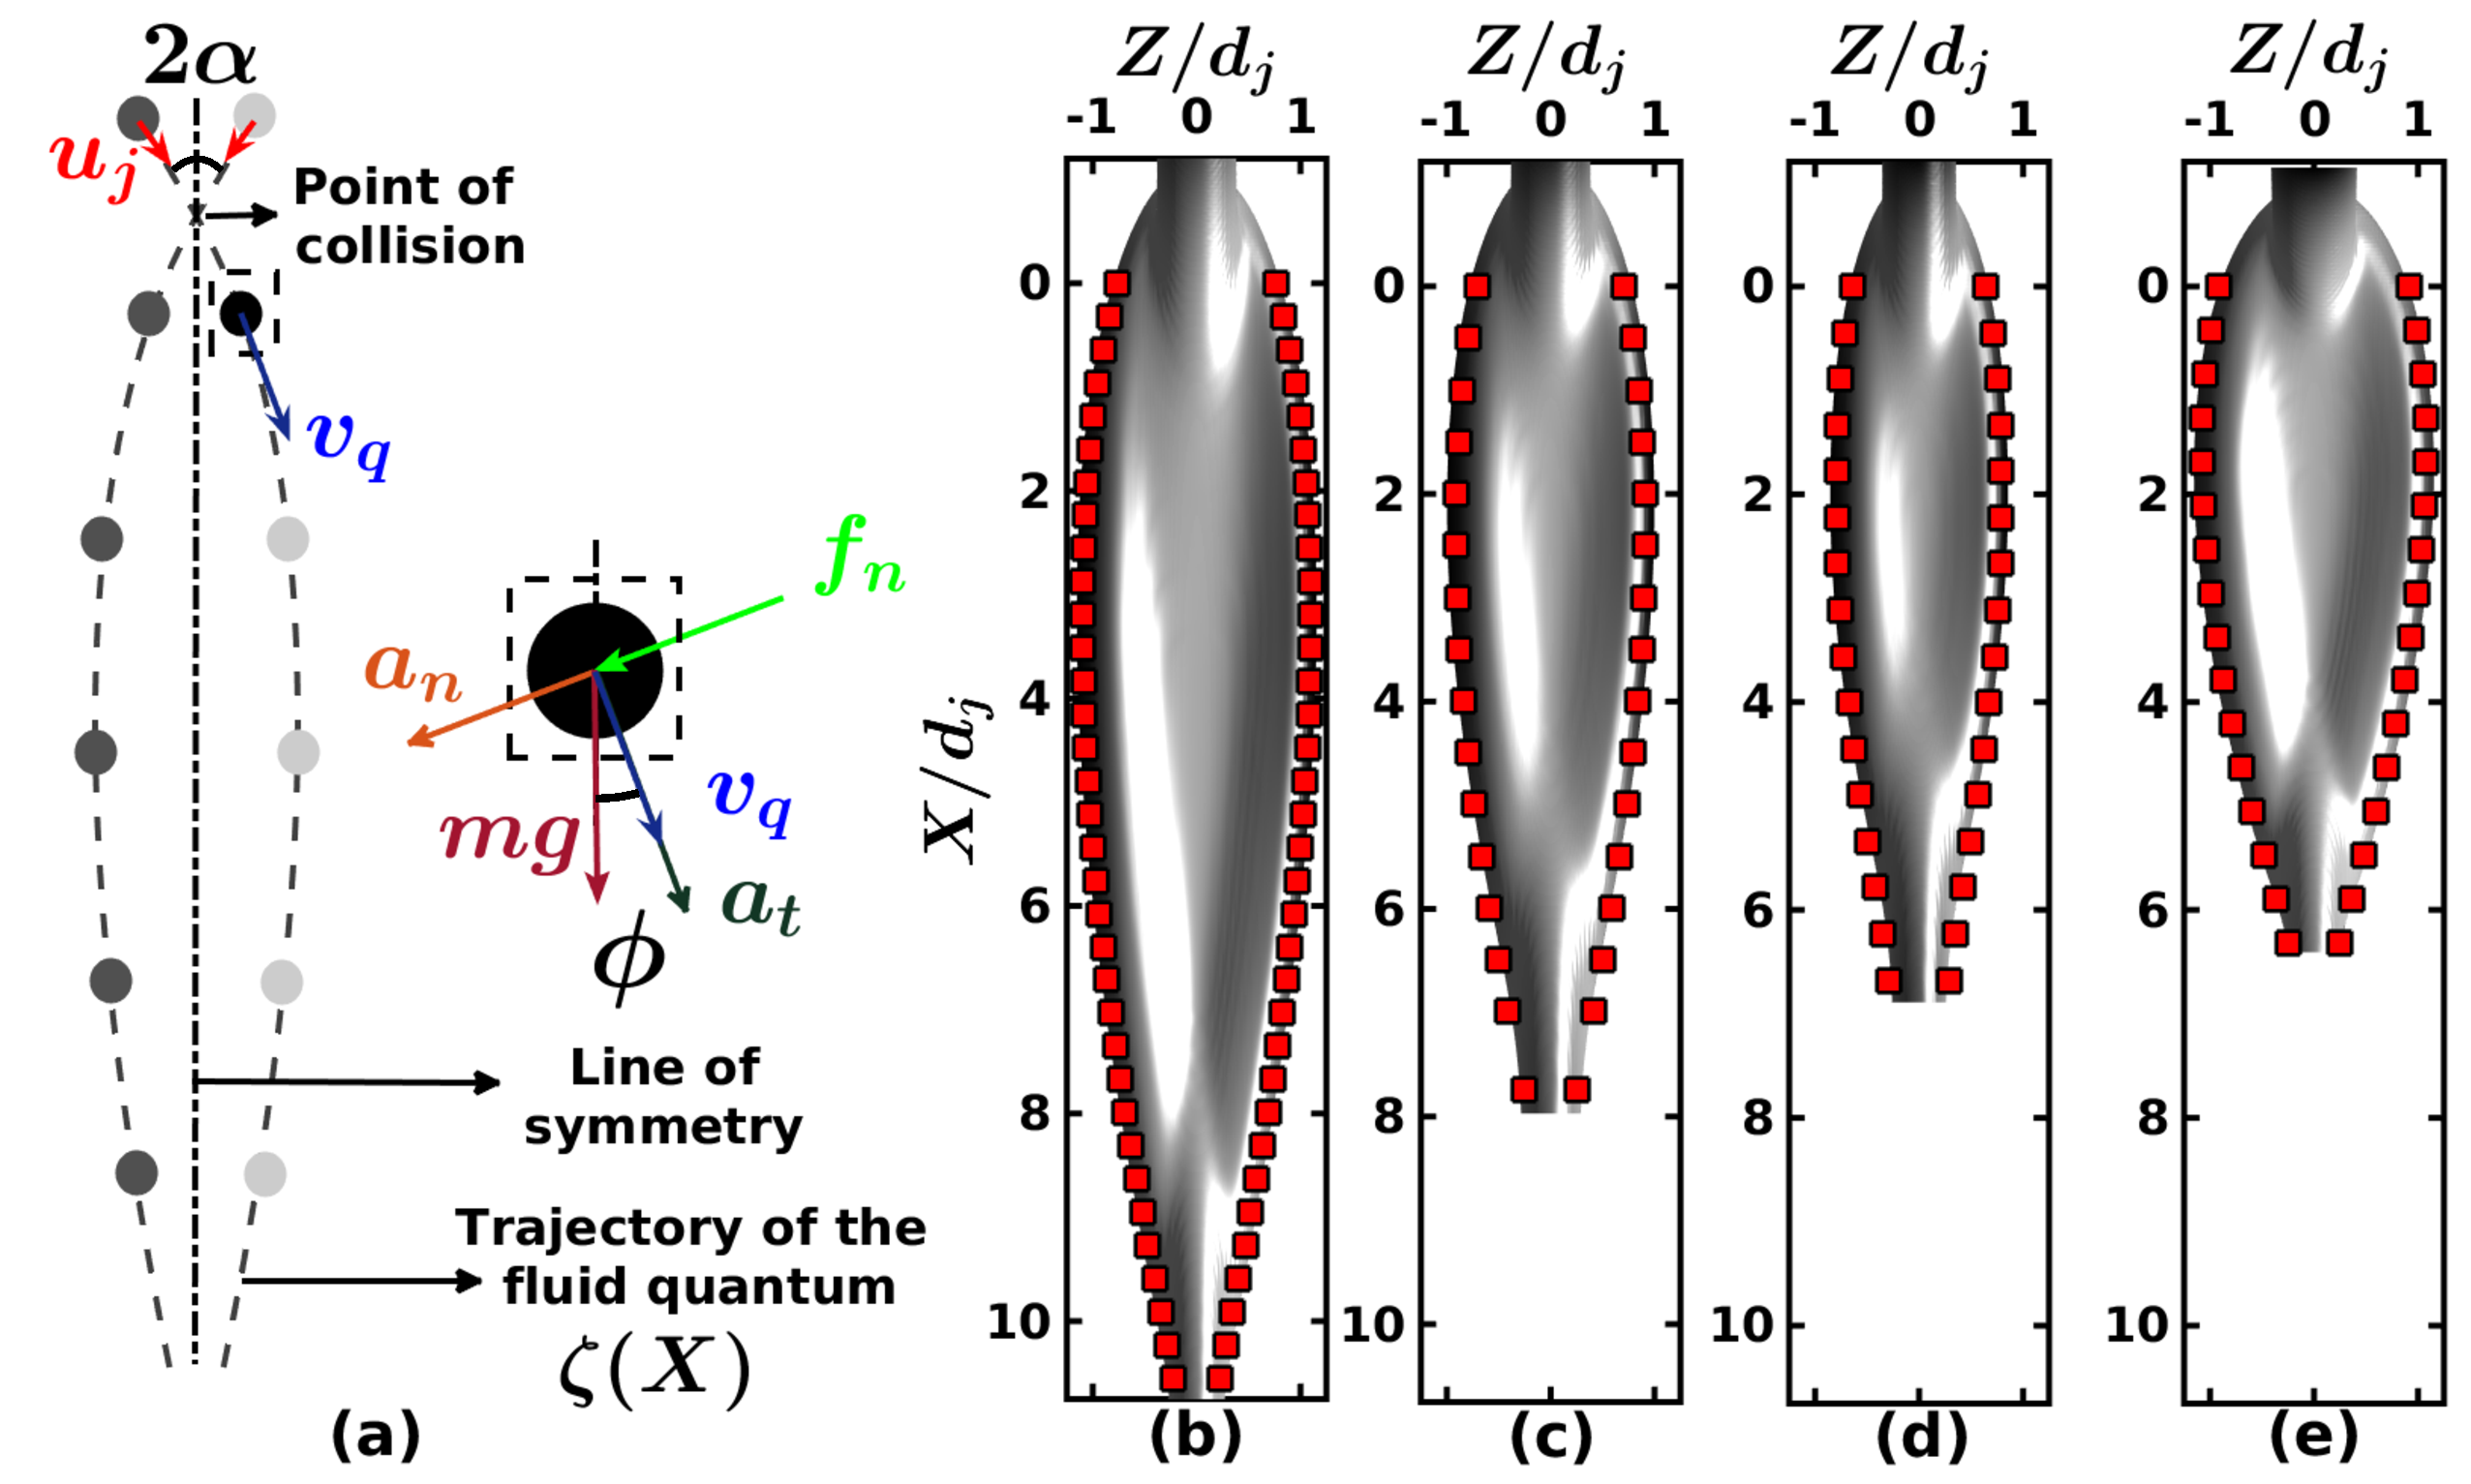
\includegraphics[width=\linewidth]{Figure10}
	\caption{}
	\label{Figure::lil1}
\end{figure}
\clearpage
\bibliographystyle{jfm}
\bibliography{chains}
\end{document}
